% Background Bias in Image Classification -- CSCI 494 Deep Learning, final report.
% Tables in tables/*.tex are generated from results/ by tools/make_report_tables.py; do not edit them by hand.
% Compile: pdflatex main && pdflatex main   (or upload the report/ folder to Overleaf).
\documentclass[11pt,a4paper]{article}

\usepackage[margin=2.3cm]{geometry}
\usepackage[T1]{fontenc}
\usepackage[utf8]{inputenc}
\usepackage{lmodern}
\usepackage{microtype}
\usepackage{amsmath,amssymb,bm}
\usepackage{graphicx}
\usepackage{booktabs}
\usepackage{longtable}
\usepackage{tabularx}
\usepackage{adjustbox}
\usepackage{array}
\usepackage{multirow}
\usepackage{xcolor}
\usepackage{caption}
\usepackage{subcaption}
\usepackage{enumitem}
\usepackage[hidelinks]{hyperref}

\graphicspath{{figures/}}
\captionsetup{font=small,labelfont=bf}
\setlist{itemsep=2pt,topsep=4pt}
\makeatletter\DeclareRobustCommand{\pp}{\,p.p\@ifnextchar.{}{.\@}}\makeatother
\newcommand{\acc}{\mathrm{Acc}}
\newcommand{\gap}{\mathrm{Gap}}
\newcommand{\flip}{\mathrm{Flip}}
\newcommand{\E}{\mathbb{E}}
\newcommand{\1}{\mathbf{1}}
\newcommand{\bootDiff}{2.3}
\newcommand{\bootLo}{1.6}
\newcommand{\bootHi}{2.9}
\newcommand{\gradcamArea}{0.59}
\newcommand{\catGapA}{4.1}
\newcommand{\catGapB}{1.1}
\newcommand{\dogGapA}{2.3}
\newcommand{\dogGapB}{0.2}

\makeatletter\let\tableinput\@@input\makeatother

\title{\textbf{Background Bias in Image Classification:}\\
Does a Breed Classifier Look at the Animal or at the Background?}
\author{Amina Abdikalyk \and Islam Sanatbek \and Tomiris Rakymbay \and Assylkhan Tleubayev\\[4pt]
\small CSCI 494: Deep Learning \quad\textbullet\quad code: \url{https://github.com/mundmina/dl_project}}
\date{November 2026}

\begin{document}
\maketitle

\begin{abstract}
Neural networks often solve a task through a \emph{shortcut}: a feature that is correlated with the label in the
training data but is not the thing we want the model to use. The background of a photo is the classic example.
We study it in a small, fully controlled setting: fine-grained recognition of 37 cat and dog breeds
(Oxford-IIIT Pet), where pixel-accurate pet masks let us replace the background of every test image with an
unrelated scene from Places365. We define four test conditions (original, background swapped, foreground only,
background only), compare a classical HOG + linear SVM baseline with five deep architectures
(ResNet-18, ResNet-18 trained from scratch, ResNet-50, ConvNeXt-T, Swin-T), and test a simple remedy:
replacing the background of a training image by a random scene with probability $p$.
A ResNet-18 fine-tuned on original images loses $2.8\pm0.7$\pp{} of test accuracy when only the background changes
($89.7\%\to86.9\%$) and changes its prediction on $8.4\%$ of the images. With background swapping ($p=0.5$) the drop
shrinks to $0.5\pm0.2$\pp{} (paired bootstrap difference \bootDiff\pp, 95\% CI [\bootLo, \bootHi]) at no cost in
accuracy on original images. The effect holds for all five architectures, an ablation shows that $p=0.25$ already
removes most of the gap, and among six training strategies (gray background, blurred background, CutMix, an
input-gradient saliency penalty with $\lambda\in\{1,10\}$, random scene swap) only the random scene swap removes it.
Linear probes show that swap training removes most background-scene information from the learned features. The
background-only condition stays close to chance for ResNet-18, so the model is \emph{distracted} by unfamiliar
backgrounds rather than reading the breed off the background. Finally, the same remedy transfers to two settings
it was not designed on: real photographs from Stanford Dogs, and the Waterbirds shortcut benchmark, where it raises
worst-group accuracy from $65\%$ to $80\%$.
\end{abstract}

\tableofcontents
\newpage

%======================================================================
\section{Introduction}
%======================================================================

\paragraph{The big problem: shortcut learning.}
A classifier is trained to minimise its error on the training data. It will use \emph{any} feature that lowers that
error, whether or not a human would call the feature relevant. If, in the training set, huskies are mostly
photographed on snow, ``white background'' predicts ``husky'' and the model may learn exactly that
\cite{ribeiro2016lime}. Geirhos et al.\ call this \emph{shortcut learning} \cite{geirhos2020shortcut}: the model
reaches high accuracy on data that looks like its training set and fails when the correlation breaks.
The same failure appears in high-stakes applications:
\begin{itemize}
  \item \textbf{Medicine.} Pneumonia detectors trained on chest X-rays from several hospitals learned to recognise
  the \emph{hospital} (from scanner-specific tokens and image statistics), which correlated with disease prevalence,
  and generalised worse to new hospitals \cite{zech2018pneumonia}.
  \item \textbf{Ecology.} Animal detectors for camera traps fail at new camera locations because they rely on the
  scenery of the locations they were trained on \cite{beery2018terra}.
  \item \textbf{Agriculture and remote sensing.} Plant-disease and land-use classifiers face the same risk when the
  field, the lighting or the region is correlated with the class.
\end{itemize}
A shortcut is invisible on a test set drawn from the same distribution as the training set: the correlation is
there as well, so the shortcut ``works''. To see it, one has to \emph{break the correlation on purpose} and measure
what happens. That is what this project does.

\paragraph{Our small, controllable case.}
We pick a task where the shortcut can be switched on and off precisely: breed classification on Oxford-IIIT Pet
\cite{parkhi2012cats}. Every image comes with a \emph{trimap} that marks the pet, the background and an uncertain
border. With the mask we can paste the pet onto a different background, remove the background entirely, or remove
the pet and keep only the background. Breeds are a fine-grained task (37 classes, some of them almost identical),
so a model has reasons to grab any extra cue, and the background of a pet photo (sofa, lawn, show ring) is a
plausible one.

\paragraph{Research questions.}
\begin{enumerate}[label=\textbf{RQ\arabic*.}]
  \item Does a standard fine-tuned CNN rely on the background to classify the breed?
  \item Does randomly replacing the background during training reduce that reliance, and what does it cost in
  ordinary accuracy?
  \item Does the answer depend on the architecture, and how does the remedy compare with other ways of handling the
  background?
  \item Does a remedy learned on synthetic composites transfer to real photographs and to a standard shortcut
  benchmark?
\end{enumerate}

\paragraph{Hypotheses (written down before training).}
\begin{itemize}
  \item[\textbf{H1.}] ResNet-18 A (trained on original images) loses noticeable accuracy when the background is
  swapped.
  \item[\textbf{H2.}] ResNet-18 B (trained with random background swap) has a smaller gap than A, at comparable
  accuracy on original images.
  \item[\textbf{H3.}] Both models lose less on foreground-only images (neutral gray background) than on swapped
  images: a neutral background carries no misleading signal, while a foreign scene can actively mislead.
\end{itemize}

\paragraph{Contributions.}
(i) A controlled evaluation protocol with four test conditions and fixed, reproducible test backgrounds drawn from
scene categories that never occur in training. (ii) A comparison of 17 trained configurations, 51 runs in total
(3 seeds each), plus a classical baseline. (iii) Statistical tests (paired bootstrap) for the main claims.
(iv) Mechanistic analyses: per-breed gaps, Grad-CAM, and linear probes of background information in the features.
(v) Two transfer studies: an external test on real photos (Stanford Dogs) and a case study on Waterbirds.

%======================================================================
\section{Related work}
%======================================================================

\textbf{Backgrounds in object recognition.} Xiao et al.\ \cite{xiao2021noise} built ImageNet-9 with variants such as
\emph{Only-FG}, \emph{Mixed-Same} (foreground on a background of the same class) and \emph{Mixed-Rand} (foreground on a
random background) and showed that ImageNet models depend on backgrounds, less so for more accurate models. Our
``swapped'' condition is their Mixed-Rand, our ``foreground only'' is their Only-FG (gray instead of black), and our
``background only'' corresponds to their Only-BG-T. Our dataset differs: a fine-grained task with exact masks.

\textbf{Shortcut learning and spurious correlations.} Geirhos et al.\ \cite{geirhos2020shortcut} give the general
framing. Beery et al.\ \cite{beery2018terra} show the location dependence of camera-trap models. Sagawa et al.\
\cite{sagawa2020dro} introduce Waterbirds (CUB birds \cite{wah2011cub} pasted onto Places scenes with a 95\%
bird--background correlation) and the \emph{worst-group accuracy} metric; they fix it with group DRO, which requires
group labels. Our remedy needs foreground masks instead of group labels.

\textbf{Fixing shortcuts.} Data-side fixes change what the model sees: background randomisation (ours, and
Mixed-Rand training in \cite{xiao2021noise}), or generic augmentation such as CutMix \cite{yun2019cutmix}.
Loss-side fixes change what the model is rewarded for: ``Right for the Right Reasons'' \cite{ross2017rrr} penalises
input gradients on regions annotated as irrelevant. We compare both families under one protocol.

\textbf{Tools.} ResNet \cite{he2016resnet}, ConvNeXt \cite{liu2022convnext}, Swin Transformer \cite{liu2021swin}, all
pretrained on ImageNet \cite{deng2009imagenet}; Places365 \cite{zhou2018places}; HOG \cite{dalal2005hog}; Grad-CAM
\cite{selvaraju2017gradcam}; linear probes \cite{alain2016probes}; DeepLabV3 \cite{chen2017deeplab}; AdamW
\cite{loshchilov2019adamw}; cosine schedules \cite{loshchilov2017sgdr}; bootstrap \cite{efron1993bootstrap};
Stanford Dogs \cite{khosla2011dogs}.

%======================================================================
\section{Data}
%======================================================================

\subsection{Oxford-IIIT Pet}
Oxford-IIIT Pet \cite{parkhi2012cats} has 7{,}349 photos of 37 breeds (12 cat, 25 dog breeds), about 200 per breed,
with an official \texttt{trainval}/\texttt{test} split. Each image has a trimap $T(u)\in\{1,2,3\}$ for every pixel
$u$: $1$ = pet, $2$ = background, $3$ = border/uncertain (usually a band of fur along the outline).

\paragraph{Splits.} The official \texttt{test} split (3{,}669 images) is our test set and was used once, at the very
end. We split the official \texttt{trainval} (3{,}680 images) into train and validation with a stratified (by
breed) 85/15 split, \texttt{random\_state=42}. Splits are made on image ids before any variant exists, so all
versions of an image stay in the same split; the code asserts that the three sets are disjoint and that every split
contains all 37 classes. The CSV files are committed to the repository and used by every model.

\begin{table}[h]
\centering\small
\begin{adjustbox}{max width=\linewidth}
\begin{tabular}{lrrrrr}
\toprule
Split & Images & Cats & Dogs & Min / max images per breed \\
\midrule
Train & 3{,}128 & 1{,}010 & 2{,}118 & 79 / 85 \\
Validation & 552 & 178 & 374 & 14 / 15 \\
Test (official) & 3{,}669 & 1{,}183 & 2{,}486 & 88 / 100 \\
\bottomrule
\end{tabular}
\end{adjustbox}
\caption{Pet splits. Classes are balanced, so chance accuracy is $1/37 = 2.7\%$.}
\label{tab:splits}
\end{table}

\paragraph{Data audit.} All 7{,}349 images and trimaps load; 3 images are RGBA and are converted to RGB; every trimap
matches its image size. On average the pet covers 30.0\% of an image (class 1), the border 11.8\% (class 3) and
the background 58.2\% (class 2); the pet fraction ranges from 0\% to 94.7\%, so a few masks are nearly empty.

\subsection{Background scenes: Places365}
Backgrounds come from the Places365 validation set \cite{zhou2018places} (36{,}500 images at $256\times256$,
100 per category). We first drop the 17 categories in which animals often appear (every category whose name contains one of
\emph{kennel, pasture, corral, barn, stable, veterinarian, pet\_shop, zoo, aquarium, ranch, farm, chicken, cattle,
hunting, fishpond, field/wild, rodeo, racecourse}), so that a pasted pet rarely lands next to another animal. The remaining 348 categories are shuffled
(seed 42) and \emph{whole categories} are assigned to three disjoint pools:

\begin{table}[h]
\centering\small
\begin{adjustbox}{max width=\linewidth}
\begin{tabular}{lrrl}
\toprule
Pool & Categories & Images & Used for \\
\midrule
\texttt{bg\_train} & 209 & 20{,}900 & random swaps during training (models B, ablation, Waterbirds B) \\
\texttt{bg\_val} & 52 & 5{,}200 & swapped validation set (monitoring only) \\
\texttt{bg\_test} & 87 & 8{,}700 & swapped test set; probing labels \\
\bottomrule
\end{tabular}
\end{adjustbox}
\caption{Background pools. Pools share no image and no scene category, so test backgrounds are
\emph{new types of scene}, not just new photos of known scenes.}
\label{tab:pools}
\end{table}

\paragraph{Fixed evaluation backgrounds.} For every validation and test image we draw one background from its pool
once (seed fixed) and store it in a manifest (\texttt{manifests/\{val,test\}\_swapped.csv}). Composites are rendered on
the fly but deterministically, so every model is evaluated on \emph{exactly the same} swapped images.

\subsection{Composition: how a swapped image is made}
Let $x\in[0,255]^{H\times W\times 3}$ be the photo and $T$ its trimap. The binary foreground is
\begin{equation}
  m(u) = \1\big[T(u)=1\big] \;\lor\; \1\big[T(u)=3\big],
  \label{eq:mask}
\end{equation}
i.e.\ the border class is counted as pet. Without it, the outer fur would be cut off and the pet would look
``shaved''. A hard mask makes a visible seam, so we soften it with a Gaussian blur of $\sigma=1.5$ px:
\begin{equation}
  \alpha = G_{\sigma}*m \;\in [0,1]^{H\times W}.
  \label{eq:alpha}
\end{equation}
A new background $b$ is scaled to cover $H\times W$ (aspect preserved) and cropped at relative offset
$o\in[0,1]^2$ (the centre $o=(0.5,0.5)$ at test time, uniformly random in training). The composite is standard alpha
blending, pixel by pixel:
\begin{equation}
  \tilde x(u) = \alpha(u)\,x(u) + \big(1-\alpha(u)\big)\,b(u).
  \label{eq:composite}
\end{equation}
Pixels with $\alpha=1$ keep the pet, pixels with $\alpha=0$ show the new scene, and the blurred band in between mixes
the two, which hides the seam.

\subsection{The four test conditions}
All four are built from the same test image with Eq.~\eqref{eq:composite}; only $b$ (and, for the last one, the roles of
the pet and the background) change. Let $g$ be a constant image with the mean ImageNet colour $(124,116,104)$.
\begin{center}\small
\begin{tabularx}{\textwidth}{lXl}
\toprule
Condition & Definition & What it tests \\
\midrule
\textbf{original} & $x$ unchanged & ordinary accuracy \\
\textbf{swapped} & $\alpha x + (1-\alpha)\,b_{\text{test}}$, $b_{\text{test}}$ from the manifest & robustness to a foreign scene \\
\textbf{fg-only} & $\alpha x + (1-\alpha)\,g$ & accuracy without any background \\
\textbf{bg-only} & $\alpha g + (1-\alpha)\,x$ & can the breed be read off the background alone? \\
\bottomrule
\end{tabularx}
\end{center}
\textbf{Why fg-only matters.} A drop on swapped images could have two causes: (a) the model relied on the original
background, or (b) the model is hurt by \emph{paste artifacts} (seams, lighting mismatch). Fg-only images have the same
paste artifacts but no misleading scene. If the fg-only drop is much smaller than the swapped drop, artifacts are not
the main cause (H3). \textbf{Why bg-only matters.} If a model scores far above chance with the pet painted over,
the background (or the pet's silhouette, which bg-only keeps) carries breed information that the model uses.

Figure~\ref{fig:gallery} in the appendix shows examples of all conditions.

\subsection{External data}
\textbf{Stanford Dogs} \cite{khosla2011dogs} has 20{,}580 photos of 120 breeds with bounding boxes. Twenty-one of its
breeds are also Pet breeds (mapping by ImageNet synset in \texttt{src/bgbias/stanford\_dogs.py}; the pit bull is
left out because Stanford has only the American Staffordshire terrier, and American bulldog, Havanese and Shiba Inu
have no counterpart). This gives 3{,}730 real photos, taken by other people in other places, with no cut-and-paste.
We evaluate two views: \emph{full} (whole photo) and \emph{crop} (the union of all annotated dog boxes, which removes
most of the background).

\textbf{Waterbirds} \cite{sagawa2020dro}: CUB-200 birds \cite{wah2011cub} pasted onto Places scenes, label
$y\in\{\text{landbird},\text{waterbird}\}$, place $a\in\{\text{land},\text{water}\}$. In train, 95\% of waterbirds sit on
water and 95\% of landbirds on land; the test set has all four (bird, place) groups. Splits: 4{,}795 train,
1{,}199 val, 5{,}794 test. Waterbirds has no masks, so we segment the bird with a pretrained DeepLabV3-ResNet50
\cite{chen2017deeplab} (class ``bird'' of the VOC label set) and use that mask in Eq.~\eqref{eq:composite}.

%======================================================================
\section{Methods}
%======================================================================

\subsection{Notation and the learning problem}
A model $f_\theta$ maps an image to logits $z=f_\theta(x)\in\mathbb{R}^{K}$, $K=37$. Class probabilities are the softmax
\begin{equation}
  p_\theta(k\mid x) = \frac{\exp z_k}{\sum_{j=1}^{K}\exp z_j},\qquad \hat y(x)=\arg\max_k z_k .
\end{equation}
All networks are trained with the cross-entropy loss on a mini-batch $\mathcal B$:
\begin{equation}
  \mathcal L_{\mathrm{CE}}(\theta) = -\frac{1}{|\mathcal B|}\sum_{(x,y)\in\mathcal B}\log p_\theta(y\mid x).
  \label{eq:ce}
\end{equation}

\subsection{The remedy: random background swap (model B)}
Each time a training image is loaded, with probability $p$ its background is replaced by a random scene:
\begin{equation}
  x' =
  \begin{cases}
    \alpha\,x + (1-\alpha)\,b, & \text{with probability } p,\quad b\sim\mathrm{Uniform}(\texttt{bg\_train}),\; o\sim U[0,1]^2,\\
    x, & \text{with probability } 1-p,
  \end{cases}
  \label{eq:swap}
\end{equation}
and then the usual augmentations are applied to $x'$ (random resized crop, horizontal flip). A new $b$ is drawn every
epoch, so the model sees each pet on many scenes. The intuition: if the background is random, it is independent of
the label, $b\perp y$, so it cannot lower the training loss, and gradient descent has no reason to use it. Keeping
$1-p$ of the images original keeps the training distribution close to the test distribution of real photos.
\textbf{Model A} is the same model, same code, same hyperparameters, with $p=0$. Within an architecture,
the configuration files of A and B differ only in \texttt{name} and \texttt{p\_swap}.

\subsection{Alternative ways to handle the background (all on ResNet-18)}
\begin{itemize}
  \item \textbf{Gray background} ($p=0.5$): $b=g$ in Eq.~\eqref{eq:swap}. Removes the background instead of
  randomising it.
  \item \textbf{Blurred background} ($p=0.5$): $b=G_{12}*x$, the image's own background blurred with radius 12 px.
  Keeps the colours of the original scene but removes its detail.
  \item \textbf{CutMix} \cite{yun2019cutmix}: a generic augmentation that does \emph{not} use masks. With probability 0.5
  per batch, each image $x_i$ is paired with another image $x_j$ of the same batch (the batch shifted by one) and a random box
$R$ is chosen; the box of $x_i$ is
  replaced by the same box of $x_j$ and the labels are mixed by area:
  \begin{equation}
    \tilde x_i = (1-M_R)\odot x_i + M_R\odot x_j,\qquad
    \tilde y_i = \lambda\, e_{y_i} + (1-\lambda)\, e_{y_j},\qquad
    \lambda = 1-\frac{|R|}{HW},
  \end{equation}
  with $\lambda\sim\mathrm{Beta}(1,1)$ before box placement (\texttt{torchvision.transforms.v2.CutMix} defaults).
  The loss is the cross-entropy with the soft target $\tilde y_i$. CutMix tests whether a generic regulariser
  is enough.
  \item \textbf{Saliency penalty} (``Right for the Right Reasons'', RRR \cite{ross2017rrr}): train on original images
  only, but penalise sensitivity to background pixels. Let
  \begin{equation}
    G = \nabla_x \sum_{k=1}^{K}\log p_\theta(k\mid x)\in\mathbb{R}^{3\times H\times W},\qquad
    E(u)=\sum_{c=1}^{3} G_c(u)^2
  \end{equation}
  be the input gradient and its energy per pixel. The penalty is the share of that energy on the background,
  \begin{equation}
    S(x) = \frac{\sum_u E(u)\,\big(1-\alpha(u)\big)}{\sum_u E(u)}\in[0,1],\qquad
    \mathcal L = \mathcal L_{\mathrm{CE}} + \lambda\,\frac{1}{|\mathcal B|}\sum_{x\in\mathcal B} S(x),
    \label{eq:rrr}
  \end{equation}
  with $\lambda\in\{1,10\}$. Because $S$ is a fraction, $\lambda$ is on the same scale as the cross-entropy. (Ross et al.\
  penalise $\sum_u (1-\alpha)E$ directly; we normalise so that the size of the gradient does not matter, only where it
  points.) Minimising $S$ needs the derivative of a gradient (``double backpropagation''), which is about twice as
  expensive; these runs use fp32, because the input gradients underflow in fp16. The image and its mask go through the
  \emph{same} random crop and flip (\texttt{torchvision.transforms.v2} joint transform).
\end{itemize}

\subsection{Architectures}
\begin{center}\small
\begin{adjustbox}{max width=\linewidth}
\begin{tabular}{llrl}
\toprule
Model & Type & Params & Initialisation (torchvision) \\
\midrule
ResNet-18 \cite{he2016resnet} & CNN, residual & 11.7\,M & \texttt{IMAGENET1K\_V1} \\
ResNet-18 scratch & same & 11.7\,M & random (Kaiming) \\
ResNet-50 \cite{he2016resnet} & CNN, bottleneck residual & 25.6\,M & \texttt{IMAGENET1K\_V2} \\
ConvNeXt-T \cite{liu2022convnext} & modern CNN (large kernels, LayerNorm) & 28.6\,M & \texttt{IMAGENET1K\_V1} \\
Swin-T \cite{liu2021swin} & vision transformer, shifted windows & 28.3\,M & \texttt{IMAGENET1K\_V1} \\
\bottomrule
\end{tabular}
\end{adjustbox}
\end{center}
In every model the ImageNet classifier is replaced by a new linear layer with 37 outputs; the rest of the network
(the \emph{backbone}) is fine-tuned. The scratch model shows what happens without ImageNet knowledge: it has to learn
everything from 3{,}128 images.

\subsection{Training protocol}
\begin{table}[h]
\centering\small
\begin{tabularx}{\textwidth}{@{}lX@{}}
\toprule
Setting & Value \\
\midrule
Input & $224\times224$, ImageNet mean/std normalisation \\
Train augmentation & (background swap, Eq.~\ref{eq:swap}) $\to$ RandomResizedCrop(224, scale $[0.7,1]$) $\to$ horizontal flip \\
Eval transform & resize shorter side to 256 $\to$ centre crop 224 \\
Optimizer & AdamW, $\beta=(0.9,0.999)$, weight decay $10^{-4}$ \\
Learning rate & backbone $10^{-4}$, new head $10^{-3}$ (two parameter groups) \\
Schedule & cosine annealing over all steps, no warm-up, $\eta_{\min}=0$ \\
Epochs / batch & 15 epochs, batch 64 ($\approx$49 steps per epoch, 735 steps) \\
Precision & mixed precision (fp16 autocast + gradient scaling); fp32 for RRR \\
Checkpoint & epoch with the best \emph{original} validation accuracy (same rule for A and B) \\
Seeds & 0, 1, 2 (Python, NumPy, PyTorch, CUDA; DataLoader generator reseeded every epoch) \\
Scratch ResNet-18 & 40 epochs, one learning rate $10^{-3}$ for all layers, weight decay $5\cdot10^{-2}$ \\
Waterbirds & ResNet-18, 2 classes, 10 epochs, otherwise as above; checkpoint by validation \emph{average} accuracy \\
\bottomrule
\end{tabularx}
\caption{Training settings. They were fixed on the validation set for ResNet-18 A and then reused unchanged for every
configuration; nothing was tuned on the test set.}
\label{tab:hparams}
\end{table}

\paragraph{AdamW.} With gradient $g_t$, AdamW keeps running averages of the gradient and its square,
\begin{equation}
  m_t=\beta_1 m_{t-1}+(1-\beta_1)g_t,\quad v_t=\beta_2 v_{t-1}+(1-\beta_2)g_t^2,\quad
  \theta_t=\theta_{t-1}-\eta_t\Big(\frac{\hat m_t}{\sqrt{\hat v_t}+\epsilon}+w\,\theta_{t-1}\Big),
\end{equation}
where $\hat m_t,\hat v_t$ are the bias-corrected averages and $w$ the weight decay, applied directly to the weights
(``decoupled''), not through the gradient as in Adam with L2 \cite{loshchilov2019adamw}.

\paragraph{Cosine schedule.} At step $t$ of $T_{\max}$ (all steps of all epochs),
\begin{equation}
  \eta_t = \eta_{\min} + \tfrac12(\eta_0-\eta_{\min})\big(1+\cos(\pi t/T_{\max})\big),
\end{equation}
so the learning rate starts at $\eta_0$ and decays smoothly to 0; each parameter group has its own $\eta_0$.

\paragraph{Why two learning rates.} The backbone already holds useful ImageNet features; a large step would destroy
them. The new head starts from random weights and needs to move fast. A $10\times$ larger rate for the head is the
standard fine-tuning compromise.

\paragraph{Checkpoint selection and the validation sets.} After every epoch we compute validation accuracy on
original images and on swapped images (backgrounds from \texttt{bg\_val}). The swapped validation accuracy is
\emph{only logged}; the checkpoint is always chosen by original validation accuracy, for A and B alike. Choosing
by swapped accuracy would select for robustness and would favour B unfairly.

\paragraph{Reproducibility.} All randomness (background choice, crop offset, augmentations, shuffling) comes from
PyTorch generators seeded from $(\text{seed},\text{epoch})$, so an interrupted run resumed from its checkpoint
continues exactly as an uninterrupted one. The baseline A/B runs were first trained in Google Colab (T4 GPU) and
later retrained from scratch on a local GPU with the same code
(test metrics agree within $0.3$\pp; e.g.\ gap of A: $2.8\to2.8$\pp, gap of B: $0.6\to0.5$\pp).

\subsection{Classical baseline: HOG + linear SVM}
Images are resized to $128\times128$ gray, and HOG \cite{dalal2005hog} features are computed with 9 orientation bins,
$8\times8$-pixel cells and $2\times2$-cell blocks, giving $15\cdot15\cdot2\cdot2\cdot9=8{,}100$ features. With 3{,}128
training images a linear SVM on 8{,}100 raw features separates the training set perfectly and overfits, so the pipeline
is StandardScaler $\to$ PCA (256 components) $\to$ LinearSVC. $C$ was chosen on validation accuracy from
$\{10^{-5},10^{-4},10^{-3},10^{-2},10^{-1}\}$; the best was $C=10^{-5}$ (validation accuracy 9.1\%), at the edge of the
grid. The baseline is trained once on original images and evaluated on the same four conditions. It is a lower bound
that shows how hard the task is without learned features.

%======================================================================
\section{Evaluation metrics and analysis methods}
%======================================================================
Let $\mathcal D=\{(x_i,y_i)\}_{i=1}^{N}$ be the test set ($N=3{,}669$) and $c\in\{\text{orig},\text{swap},\text{fg},\text{bg}\}$
a condition; $x_i^{(c)}$ is image $i$ under condition $c$.

\paragraph{Accuracy and macro F1.}
\begin{equation}
  \acc_c = \frac1N\sum_{i=1}^{N}\1\big[\hat y(x_i^{(c)})=y_i\big],\qquad
  \mathrm{F1}^{\text{macro}}_c = \frac1K\sum_{k=1}^{K}\frac{2P_kR_k}{P_k+R_k},
\end{equation}
where $P_k$ and $R_k$ are precision and recall of class $k$. Classes are balanced, so the two agree closely
(Table~\ref{tab:f1}); we report accuracy in the main text.

\paragraph{Robustness gap.} The accuracy lost when only the background changes:
\begin{equation}
  \gap_{\text{swap}} = \acc_{\text{orig}}-\acc_{\text{swap}},\qquad \gap_{\text{fg}} = \acc_{\text{orig}}-\acc_{\text{fg}}.
\end{equation}
It is reported in percentage points (p.p.). A gap must be read together with the accuracy: a weak model can have a small
gap simply because it is wrong everywhere.

\paragraph{Flip rate.} The share of images whose prediction changes when only the background changes:
\begin{equation}
  \flip_{\text{swap}} = \frac1N\sum_{i=1}^{N}\1\big[\hat y(x_i^{(\text{swap})})\neq\hat y(x_i^{(\text{orig})})\big].
\end{equation}
The gap counts only net changes: an image that becomes wrong and another that becomes right cancel out. The flip rate
counts both, so $\flip\ge|\gap|$ and it measures how \emph{stable} the decision is, regardless of correctness.

\paragraph{Mean and spread over seeds.} Every deep configuration is trained with 3 seeds $s$; tables show
$\bar m\pm s_m$ with the sample standard deviation $s_m=\sqrt{\tfrac{1}{n-1}\sum_s (m_s-\bar m)^2}$, $n=3$. This spread
measures training randomness (initialisation of the head, data order, augmentations), not test-set sampling noise.

\paragraph{Paired bootstrap for the difference of gaps.} To test H2 we need the uncertainty of
$\gap(A)-\gap(B)$ due to the finite test set. For every test image $i$, average over seeds the per-image gap
\begin{equation}
  d_i^{M} = \frac13\sum_{s}\Big(\1[\hat y^{M,s}(x_i^{(\text{orig})})=y_i]-\1[\hat y^{M,s}(x_i^{(\text{swap})})=y_i]\Big),
  \qquad \Delta_i = d_i^{A}-d_i^{B},
\end{equation}
so that $\bar\Delta=\frac1N\sum_i\Delta_i=\gap(A)-\gap(B)$. We draw $n_{\text{boot}}=2{,}000$ bootstrap samples of $N$ indices with
replacement, compute the mean $\bar\Delta^{*}$ of each resample, and report the 2.5th and 97.5th percentiles as a 95\% confidence
interval \cite{efron1993bootstrap}. The bootstrap is \emph{paired}: A and B are resampled on the same images, so
image difficulty cancels out. The same procedure gives confidence intervals for accuracy differences on Stanford Dogs.

\paragraph{Grad-CAM and the share of attention on the pet.} For ResNet-18, Grad-CAM \cite{selvaraju2017gradcam} uses
the activations $A^k\in\mathbb{R}^{7\times7}$ of the $k$-th channel of the last convolutional block (\texttt{layer4}) and
the gradient of the predicted class score $z_{\hat y}$:
\begin{equation}
  w_k=\frac{1}{49}\sum_{i,j}\frac{\partial z_{\hat y}}{\partial A^k_{ij}},\qquad
  \mathrm{CAM}=\mathrm{ReLU}\Big(\sum_k w_k A^k\Big),
\end{equation}
upsampled bilinearly to $224\times224$ and scaled to $[0,1]$. We summarise a map by the share of its mass on the pet,
\begin{equation}
  \text{CAM-on-pet}=\frac{\sum_u \mathrm{CAM}(u)\,\alpha(u)}{\sum_u \mathrm{CAM}(u)},
\end{equation}
using the mask cropped exactly like the image. It is computed on 500 test images for every seed; the pet covers on
average \gradcamArea{} of those crops, so a map that ignored the mask would score about \gradcamArea.

\paragraph{Linear probe of background information.} How much does a model's internal representation know about the
background? We take the penultimate features $h(x)$ (the input of the classifier) of every \emph{swapped} test image
and train a linear classifier to predict the Places365 \emph{scene category} of its background (87 categories,
chance $1/87=1.1\%$). The probe is StandardScaler $\to$ PCA(128) $\to$ multinomial logistic regression ($C=0.5$),
scored by 5-fold stratified cross-validation. Test backgrounds were assigned at random, so they carry no information
about the breed: a model that keeps this information in its features spends capacity on something useless for the
task, which is the representational side of background reliance \cite{alain2016probes}. As references we probe the
same architectures with ImageNet weights before fine-tuning and a randomly initialised ResNet-18.

\paragraph{External test on Stanford Dogs.} Each model predicts over all 37 Pet classes (a cat prediction is an error).
We also report a dog-restricted accuracy where the argmax is taken over the 21 present breeds only. \emph{Caveat:}
Stanford Dogs is built from ImageNet images, so ImageNet-pretrained backbones have seen these photos (with ImageNet
labels) during pretraining. This inflates absolute numbers but affects A and B equally, so the A--B comparison is
fair; the scratch models never saw them.

\paragraph{Worst-group accuracy (Waterbirds).} With groups $g=(y,a)$,
\begin{equation}
  \acc_g=\frac{1}{|\mathcal D_g|}\sum_{i\in\mathcal D_g}\1[\hat y_i=y_i],\qquad
  \text{WGA}=\min_{g}\acc_g,\qquad \text{Avg}=\frac1N\sum_i\1[\hat y_i=y_i].
\end{equation}
A model that uses the place as a shortcut fails on the rare groups (waterbird on land, landbird on water), so WGA is the
number that exposes it. Group labels are used only for evaluation, never for training or checkpoint selection.

%======================================================================
\section{Results}
%======================================================================

\subsection{Main experiment: ResNet-18 A vs B (H1--H3)}

\begin{table}[h]
\centering\small
\setlength{\tabcolsep}{4pt}
\begin{adjustbox}{max width=\linewidth}
\begin{tabular}{lcccccccc}
\toprule
 & & \multicolumn{4}{c}{Test accuracy (\%)} & \multicolumn{2}{c}{Gap (p.p.)} & Flip \\
\cmidrule(lr){3-6}\cmidrule(lr){7-8}
Model & Seeds & Original & Swapped & Fg-only & Bg-only & swap & fg & swap (\%) \\
\midrule
\tableinput tables/main_all.tex 
\bottomrule
\end{tabular}
\end{adjustbox}
\caption{All configurations on the Pet test set (mean $\pm$ std over 3 seeds; HOG is deterministic).
Chance accuracy is 2.7\%. Gap = original $-$ condition; flip = share of predictions that change.}
\label{tab:main}
\end{table}

\begin{figure}[h]
\centering
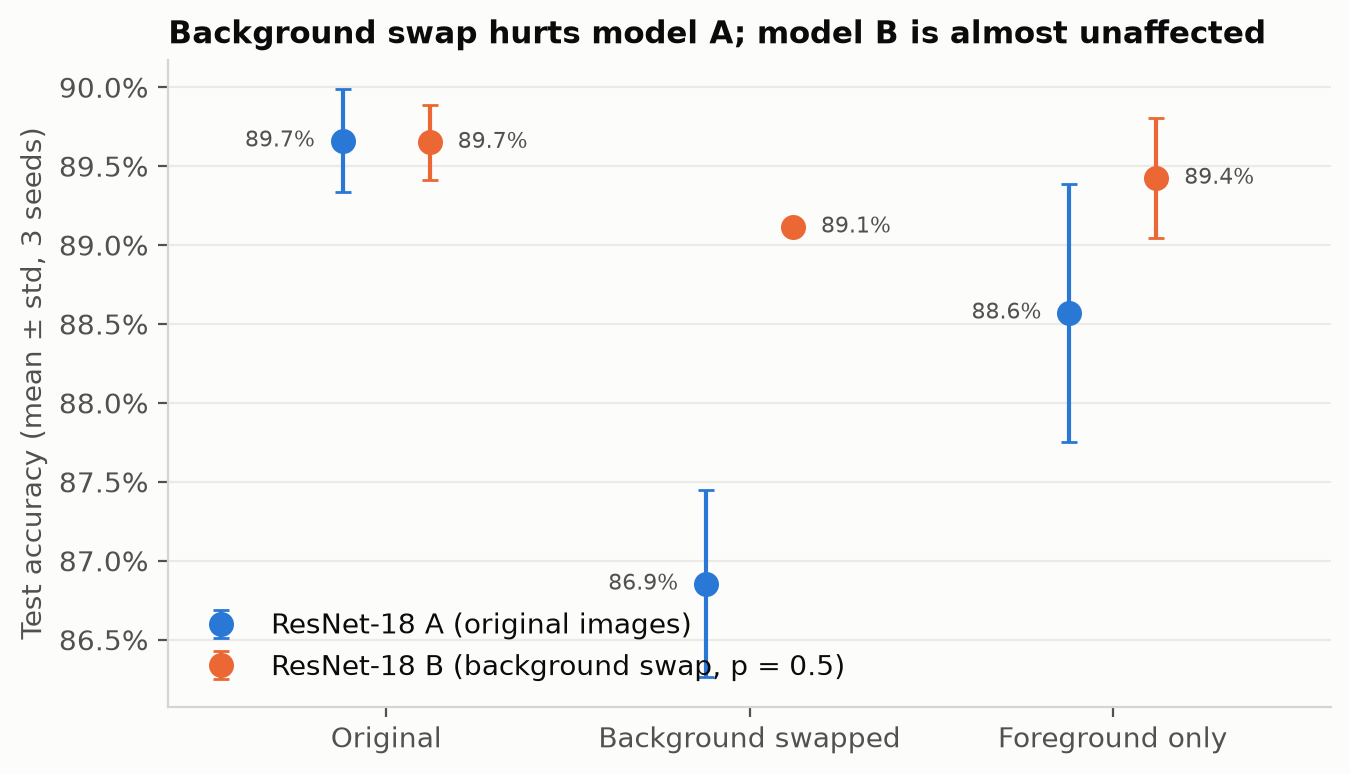
\includegraphics[width=0.72\textwidth]{fig1_accuracy_by_condition}
\caption{Test accuracy of ResNet-18 A and B under three conditions (mean $\pm$ std over 3 seeds). Both models are
equally accurate on original images; only A loses accuracy when the background is swapped.}
\label{fig:main}
\end{figure}

\paragraph{H1 confirmed.} ResNet-18 A drops from $89.7\%$ to $86.9\%$ on swapped images, a gap of $2.8\pm0.7$\pp{},
and $8.4\%$ of its predictions change (Table~\ref{tab:main}, Fig.~\ref{fig:main}). The pet is pixel-for-pixel
identical in both images; only the scene behind it differs.

\paragraph{H2 confirmed.} ResNet-18 B has the same original accuracy ($89.7\%$) but a gap of only $0.5\pm0.2$\pp{}
and a flip rate of $3.7\%$, less than half of A's. The paired bootstrap gives $\gap(A)-\gap(B)=\bootDiff$\pp{}, 95\% CI
[\bootLo, \bootHi]; none of the 2{,}000 bootstrap samples is $\le0$. Background swapping costs nothing on original
images.

\paragraph{H3 confirmed.} Both models lose less on fg-only images than on swapped ones (A: $1.1$ vs $2.8$\pp;
B: $0.2$ vs $0.5$\pp). Fg-only images have the same paste seams as swapped ones, so A's swapped drop is mostly caused
by the foreign scene, not by artifacts.

\paragraph{Background only is near chance.} With the pet painted over, A reaches $3.6\%$ and B $3.0\%$, barely above
chance (2.7\%). So the ResNet-18 does \emph{not} read the breed off the background. Together with H1 this means
the model is \emph{distracted} by an unfamiliar background (the scene pushes the features away from where the
classifier expects them) rather than exploiting a learned breed--background association. Note that this is the more
benign kind of background reliance; in Waterbirds (Section~\ref{sec:waterbirds}) the background \emph{is} predictive
and the failure is much larger.

\paragraph{HOG + SVM} reaches only $9.8\%$ on original images ($3.6\times$ chance), confirming that the task needs learned
features. Its flip rate of $74\%$ shows that its predictions are essentially unstable; its small gap ($1.3$\pp) is
meaningless at this accuracy.

\subsection{How much swapping is needed? Ablation over $p$}
\begin{table}[h]
\centering\small
\begin{adjustbox}{max width=\linewidth}
\begin{tabular}{cccccc}
\toprule
$p$ & Original (\%) & Swapped (\%) & Fg-only (\%) & Gap swap (p.p.) & Flip (\%) \\
\midrule
\tableinput tables/ablation.tex 
\bottomrule
\end{tabular}
\end{adjustbox}
\caption{ResNet-18 with swap probability $p$ (3 seeds each); $p=0$ is A, $p=0.5$ is B.}
\label{tab:ablation}
\end{table}
\begin{figure}[h]
\centering
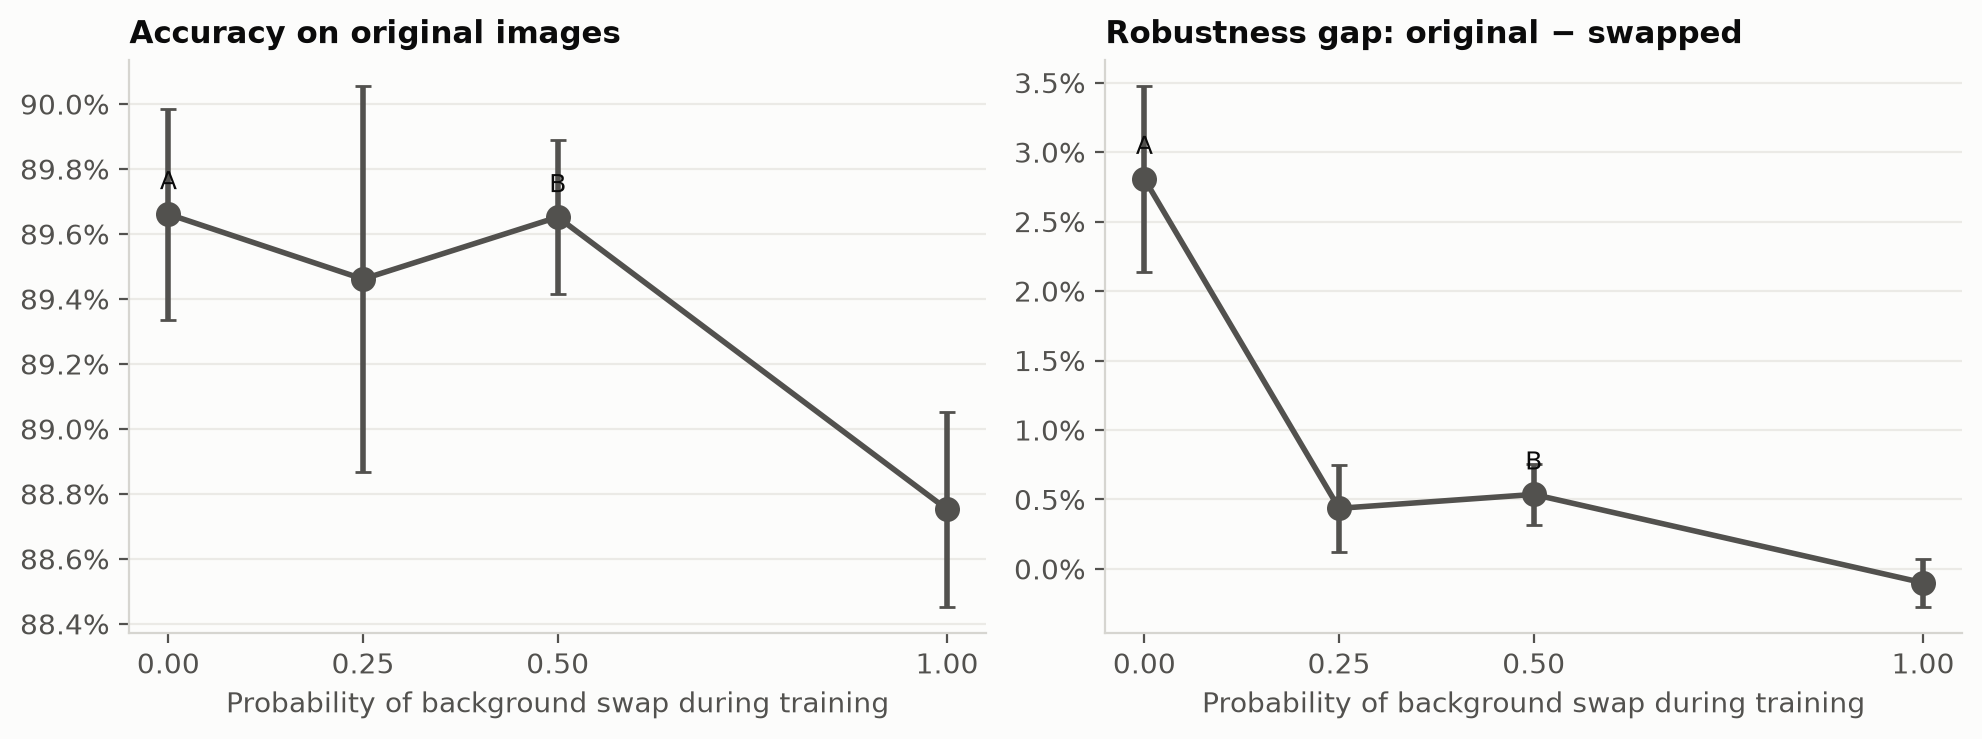
\includegraphics[width=0.95\textwidth]{fig2_ablation_p}
\caption{Accuracy and gap as a function of the swap probability $p$.}
\label{fig:ablation}
\end{figure}
Already $p=0.25$ removes almost the whole gap ($2.8\to0.4$\pp, Table~\ref{tab:ablation}, Fig.~\ref{fig:ablation}).
Original accuracy stays within $\pm0.6$\pp, which is the size of the seed spread, up to $p=0.5$; at $p=1$ (the model
never sees a real background) it is $0.9$\pp{} lower and the gap is slightly negative ($-0.1$\pp): the model is now
\emph{better} on composites than on real photos, because composites are its training distribution.
$p=0.5$ is the best compromise: highest original accuracy and lowest flip rate.

\subsection{Does it depend on the architecture?}
\begin{table}[h]
\centering\small
\setlength{\tabcolsep}{4pt}
\begin{adjustbox}{max width=\linewidth}
\begin{tabular}{llcccccc}
\toprule
Architecture & & Original (\%) & Swapped (\%) & Gap (p.p.) & Flip (\%) & Bg-only (\%) & Gap A$-$B [95\% CI] \\
\midrule
\tableinput tables/architectures.tex 
\bottomrule
\end{tabular}
\end{adjustbox}
\caption{Five architectures, A ($p=0$) vs B ($p=0.5$), 3 seeds each. The last column is the paired-bootstrap
difference of gaps.}
\label{tab:arch}
\end{table}
\begin{figure}[h]
\centering
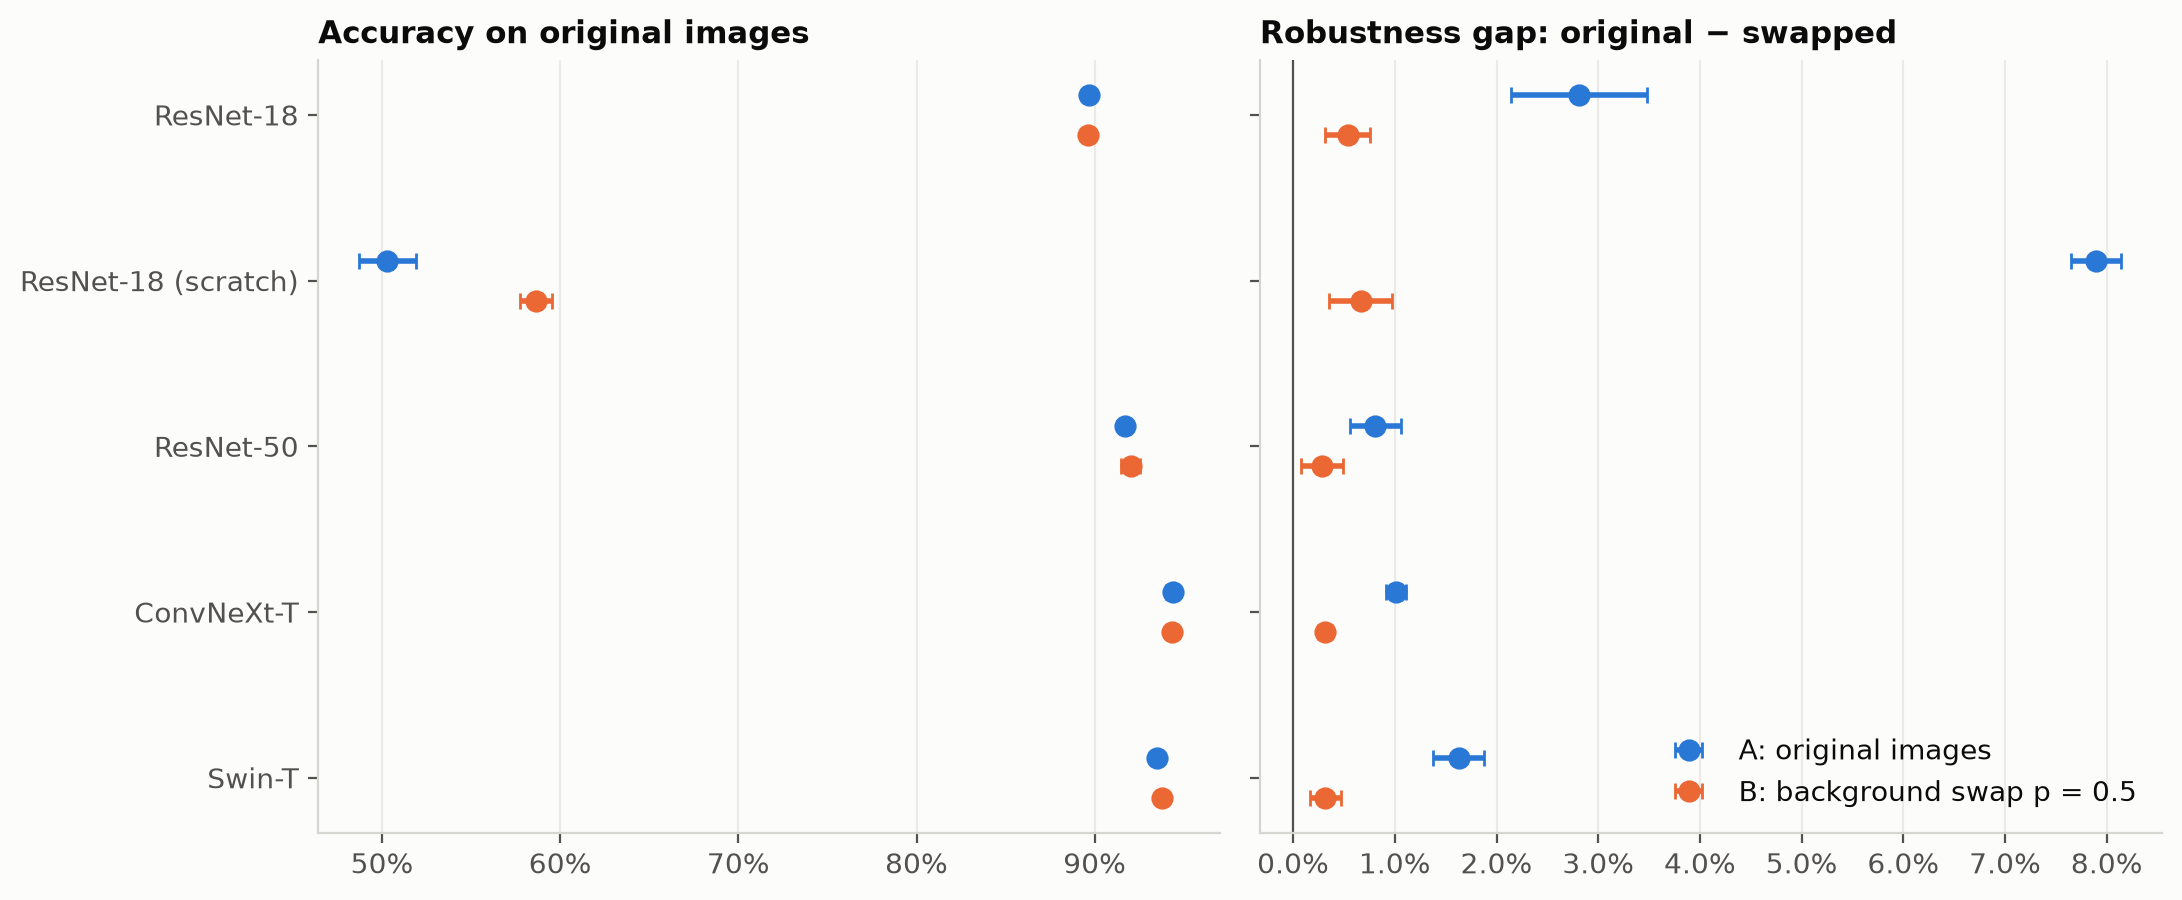
\includegraphics[width=\textwidth]{fig5_architectures}
\caption{Original accuracy (left) and robustness gap (right) for five architectures.}
\label{fig:arch}
\end{figure}
Background swapping lowers the gap for every architecture, and every bootstrap interval excludes zero
(Table~\ref{tab:arch}, Fig.~\ref{fig:arch}). Three patterns stand out:
\begin{enumerate}
  \item \textbf{Stronger models depend less on the background.} The gap of A falls from $2.8$\pp{} (ResNet-18) to
  $0.8$--$1.6$\pp{} for ResNet-50, ConvNeXt-T and Swin-T, matching the observation of Xiao et al.\ that more accurate
  models are less background-sensitive \cite{xiao2021noise}. B still cuts the remaining gap by a factor of 3--5 and
  halves the flip rate.
  \item \textbf{Without pretraining the dependence is largest.} The scratch ResNet-18 is a weak model ($50\%$) with a
  $7.9$\pp{} gap and a $45\%$ flip rate: without ImageNet features, the background is an easy statistic to fit.
  Here swapping is also a strong regulariser: B improves original accuracy by $8.4$\pp{} and reduces the gap to
  $0.7$\pp. Its fg-only accuracy is even higher than its original accuracy.
  \item \textbf{Bg-only rises with model strength.} ConvNeXt-T and Swin-T reach $7$--$10\%$ on bg-only images,
  3--4$\times$ chance, and swapping barely lowers it. Since bg-only images keep the \emph{silhouette} of the pet (the
  painted region has its exact shape), and swapping does not remove silhouette information, we attribute most of this
  to shape, not scenery (see Section~\ref{sec:discussion}).
\end{enumerate}

\subsection{Comparison of strategies for handling the background}
\begin{table}[h]
\centering\small
\begin{adjustbox}{max width=\linewidth}
\begin{tabular}{lccccc}
\toprule
Method (ResNet-18) & Original (\%) & Swapped (\%) & Fg-only (\%) & Gap (p.p.) & Flip (\%) \\
\midrule
\tableinput tables/methods.tex 
\bottomrule
\end{tabular}
\end{adjustbox}
\caption{Six ways to train ResNet-18 with respect to the background, 3 seeds each.}
\label{tab:methods}
\end{table}
\begin{figure}[h]
\centering
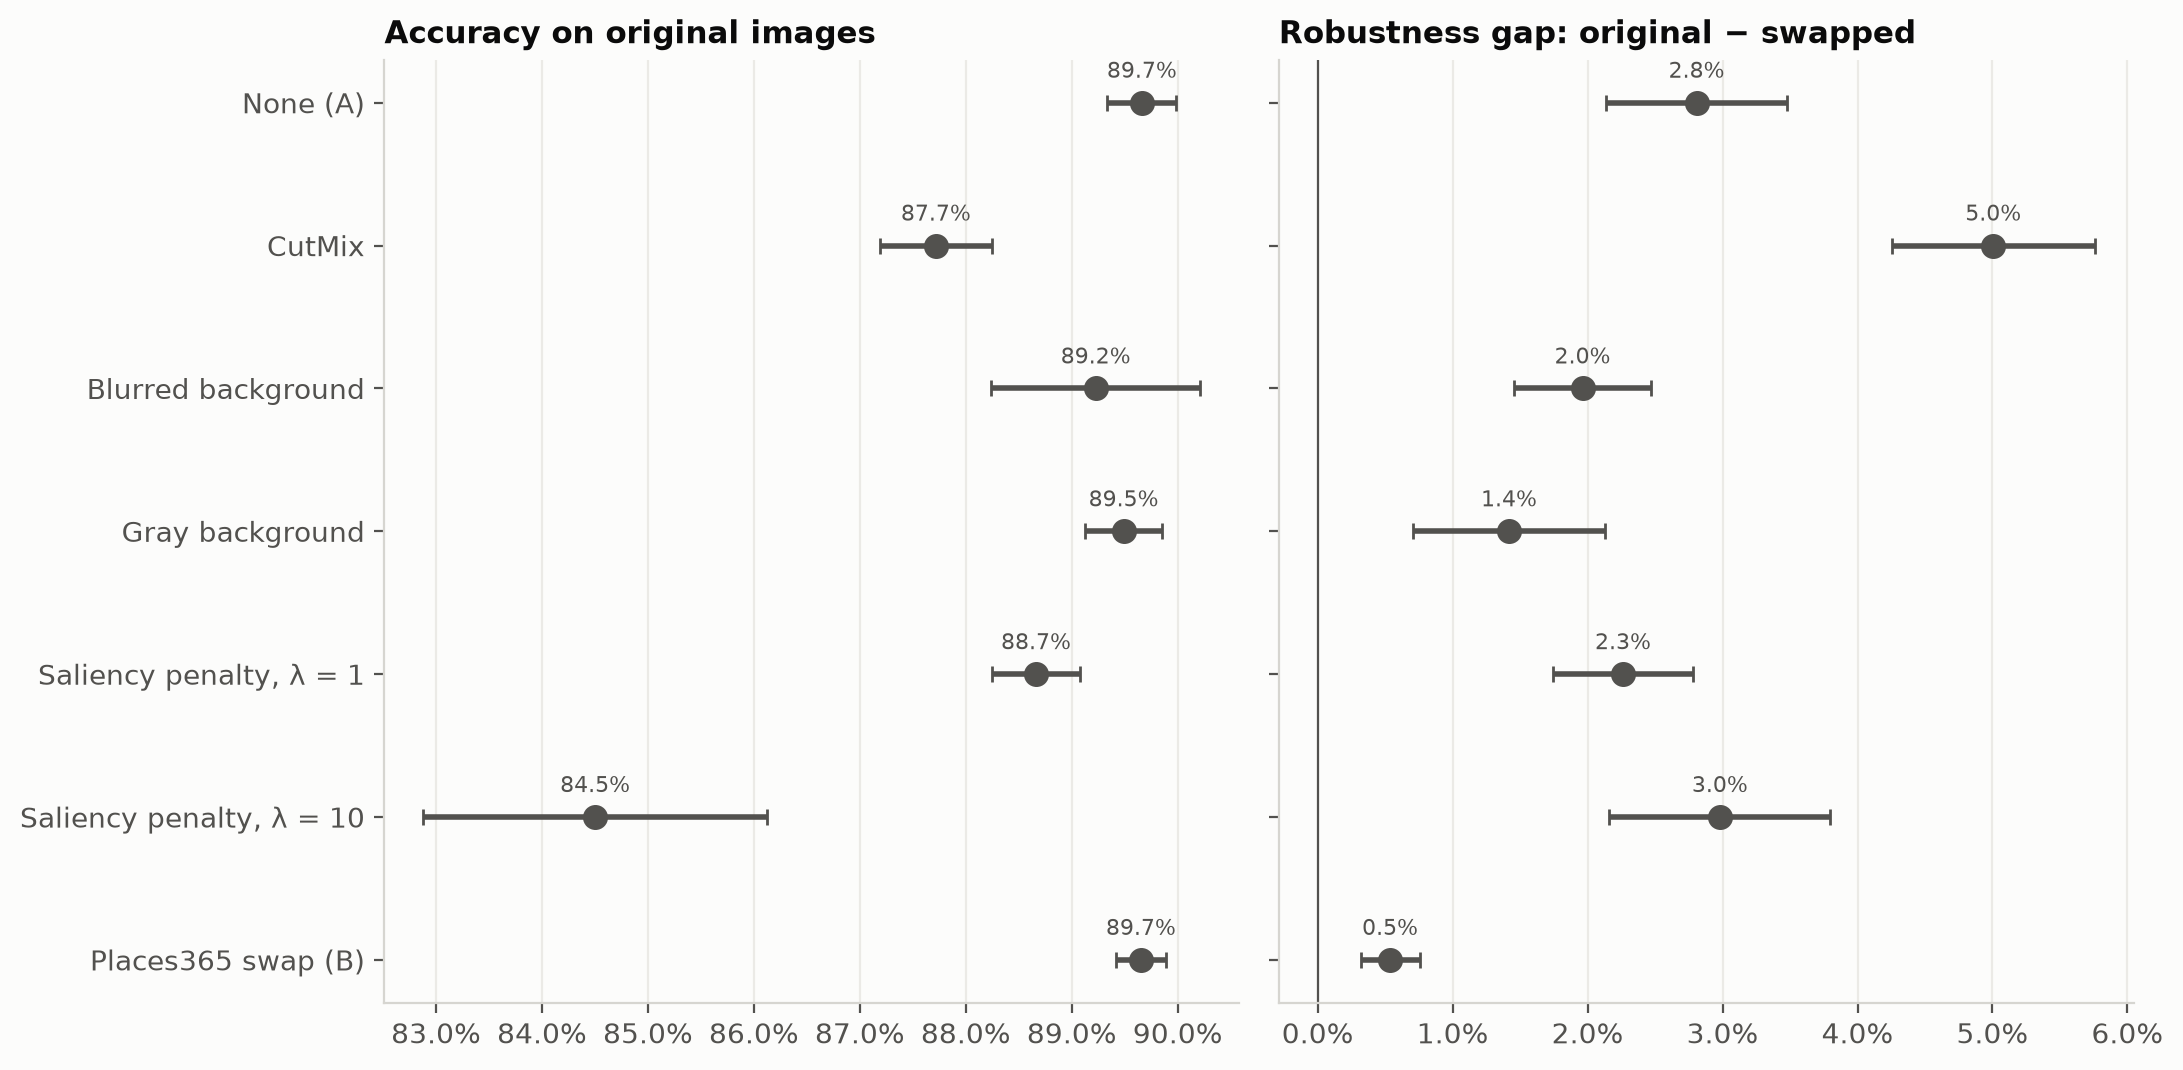
\includegraphics[width=0.95\textwidth]{fig6_methods}
\caption{Original accuracy and robustness gap of the training strategies.}
\label{fig:methods}
\end{figure}
Only the random scene swap removes the gap (Table~\ref{tab:methods}, Fig.~\ref{fig:methods}):
\begin{itemize}
  \item \textbf{Gray} ($1.4$\pp) and \textbf{blurred} ($2.0$\pp) backgrounds help partially. They teach the model to
  work without a background, but never show it a \emph{misleading} one, which is what the swapped test contains.
  \item \textbf{CutMix makes it worse} (gap $5.0$\pp, flip $14.3\%$, original $-2.0$\pp). CutMix pastes rectangles from
  other images \emph{over} the pet too and mixes the labels by area, so it does not separate pet from background;
  it seems to make the model more sensitive to local content anywhere in the image.
  \item \textbf{The saliency penalty does not help}: $\lambda=1$ gives $2.3$\pp{} (within the seed spread of A),
  $\lambda=10$ gives $3.0$\pp{} and costs $5.2$\pp{} of original accuracy. The penalty is minimised during training (for seed 0 the
  background share of the gradient energy is $6.9\%$ for $\lambda=1$ and $3.5\%$ for $\lambda=10$ in the last
  epoch, against a background area of about 60\%), but a small input gradient on the background is a \emph{local} property at the training images; it does not
  stop a large, structured change of the background from moving the features.
\end{itemize}

\subsection{Which breeds depend on the background?}
\begin{table}[h]
\centering\small
\begin{adjustbox}{max width=\linewidth}
\begin{tabular}{llrr}
\toprule
Breed & Species & Gap A (p.p.) & Gap B (p.p.) \\
\midrule
\tableinput tables/per_breed.tex 
\bottomrule
\end{tabular}
\end{adjustbox}
\caption{The 12 breeds with the largest $|\text{gap}|$ for ResNet-18 A (average over seeds; 88--100 test images per
breed, so one image $\approx1$\pp). Negative = more accurate on swapped images.}
\label{tab:breeds}
\end{table}
\begin{figure}[h]
\centering
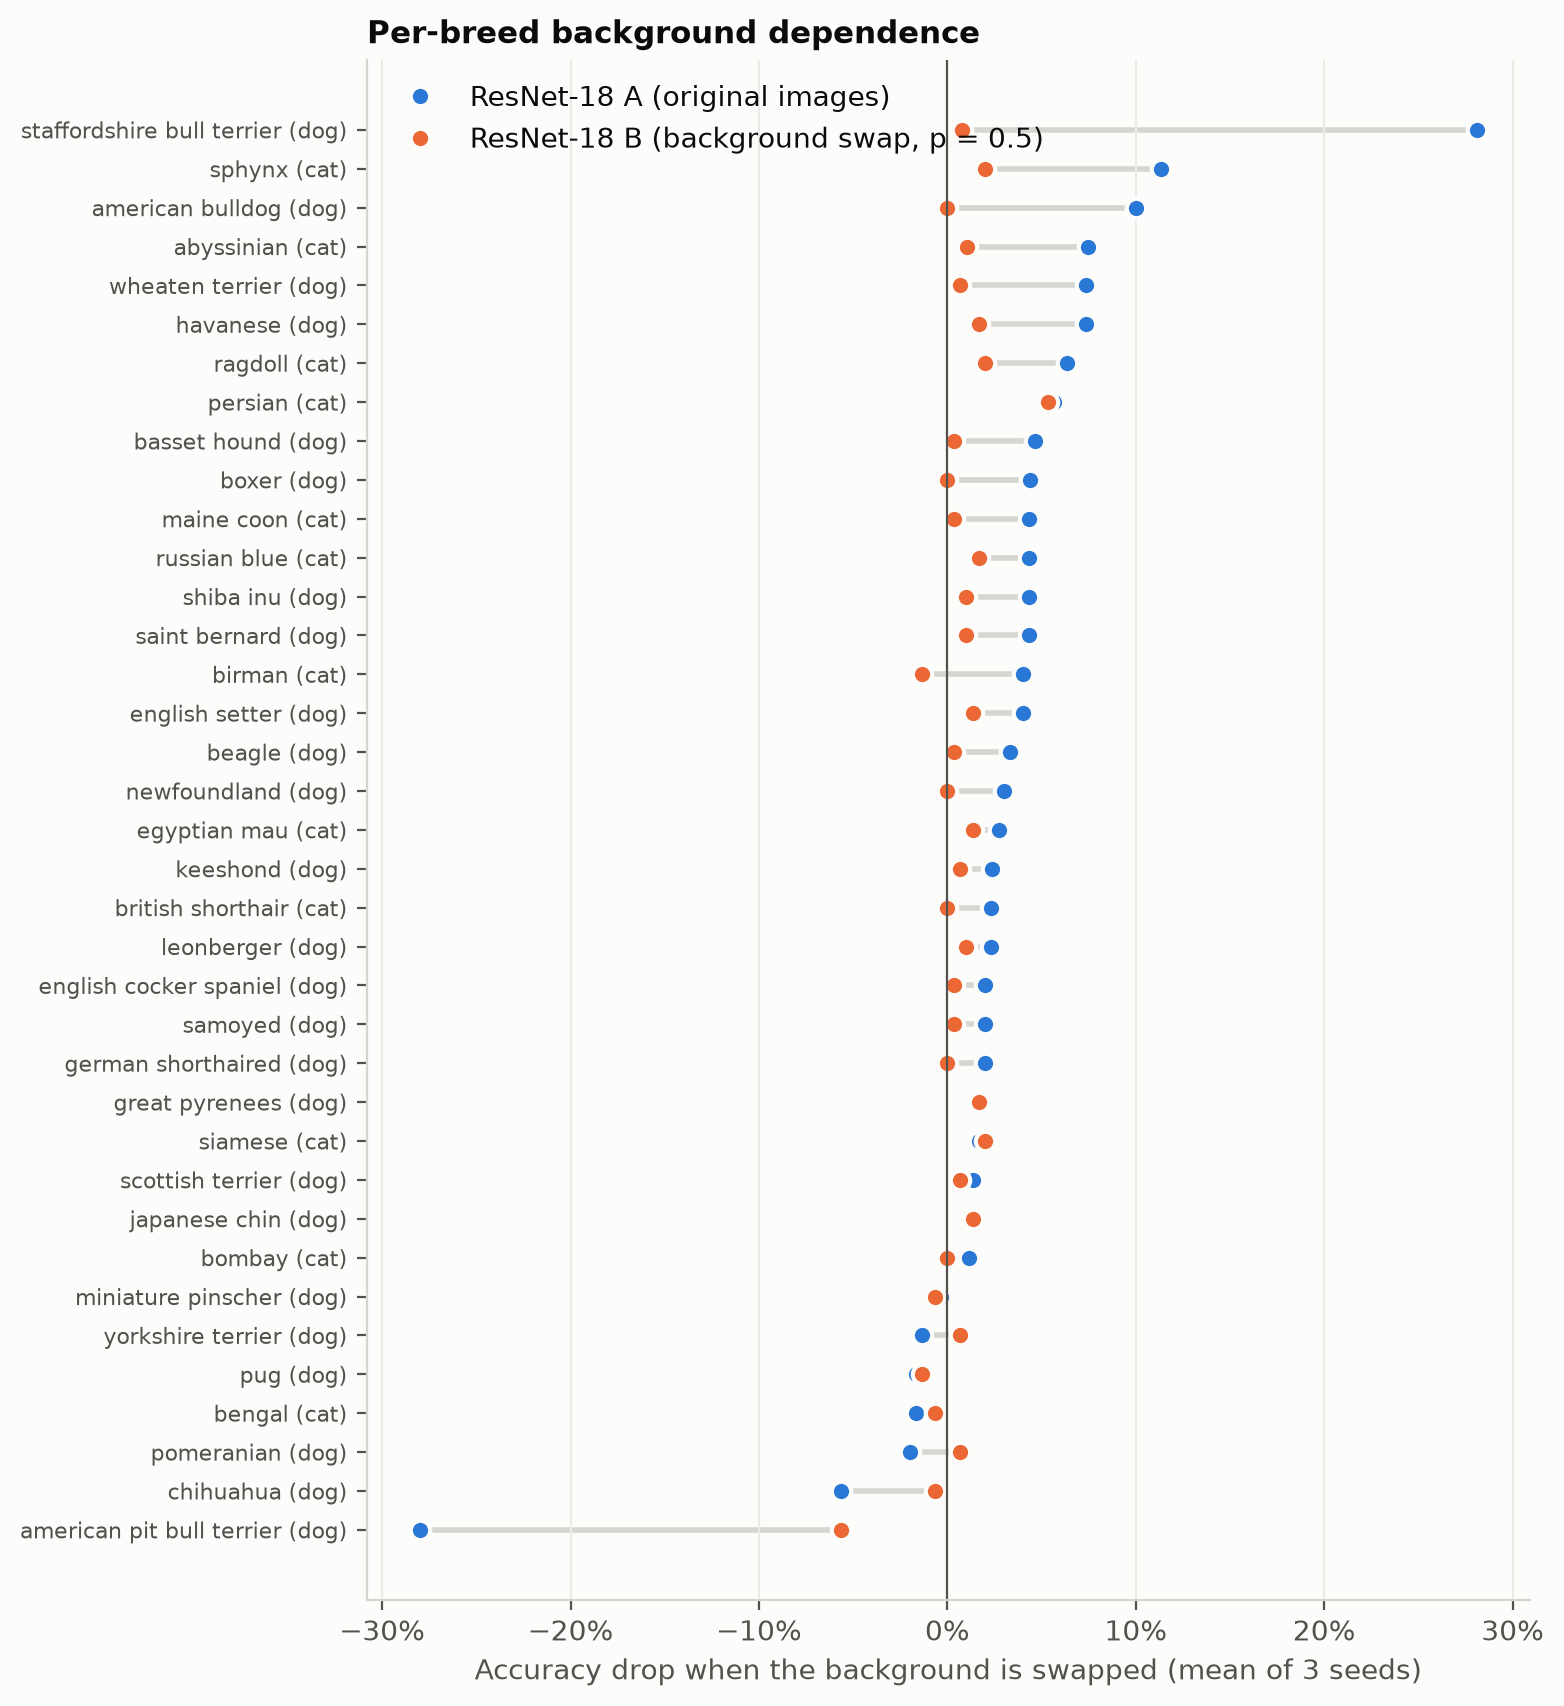
\includegraphics[width=0.7\textwidth]{fig3_per_breed_gap}
\caption{Per-breed gap of A and B.}
\label{fig:breeds}
\end{figure}
The largest effect is a \emph{pair}: Staffordshire bull terrier ($+28$\pp) and American pit bull terrier ($-28$\pp).
These two breeds look almost the same, and on swapped images A moves many Staffordshire terriers to ``pit bull''.
So for visually ambiguous breeds the background \emph{was} tipping the decision. B shrinks both to
$+0.7$ and $-5.7$\pp. On average cats have a larger gap than dogs for A (\catGapA{} vs \dogGapA\pp; B: \catGapB{} vs
\dogGapB\pp), e.g.\ Sphynx ($+11.3$\pp) and Abyssinian ($+7.5$\pp).

\subsection{Where do the models look? Grad-CAM}
\begin{table}[h]
\centering\small
\begin{adjustbox}{max width=\linewidth}
\begin{tabular}{lcc}
\toprule
Model & CAM-on-pet, original & CAM-on-pet, swapped \\
\midrule
\tableinput tables/gradcam.tex 
\bottomrule
\end{tabular}
\end{adjustbox}
\caption{Share of Grad-CAM mass on the pet (500 test images $\times$ 3 seeds). Pet area $\approx$ \gradcamArea.}
\label{tab:gradcam}
\end{table}
\begin{figure}[p]
\centering
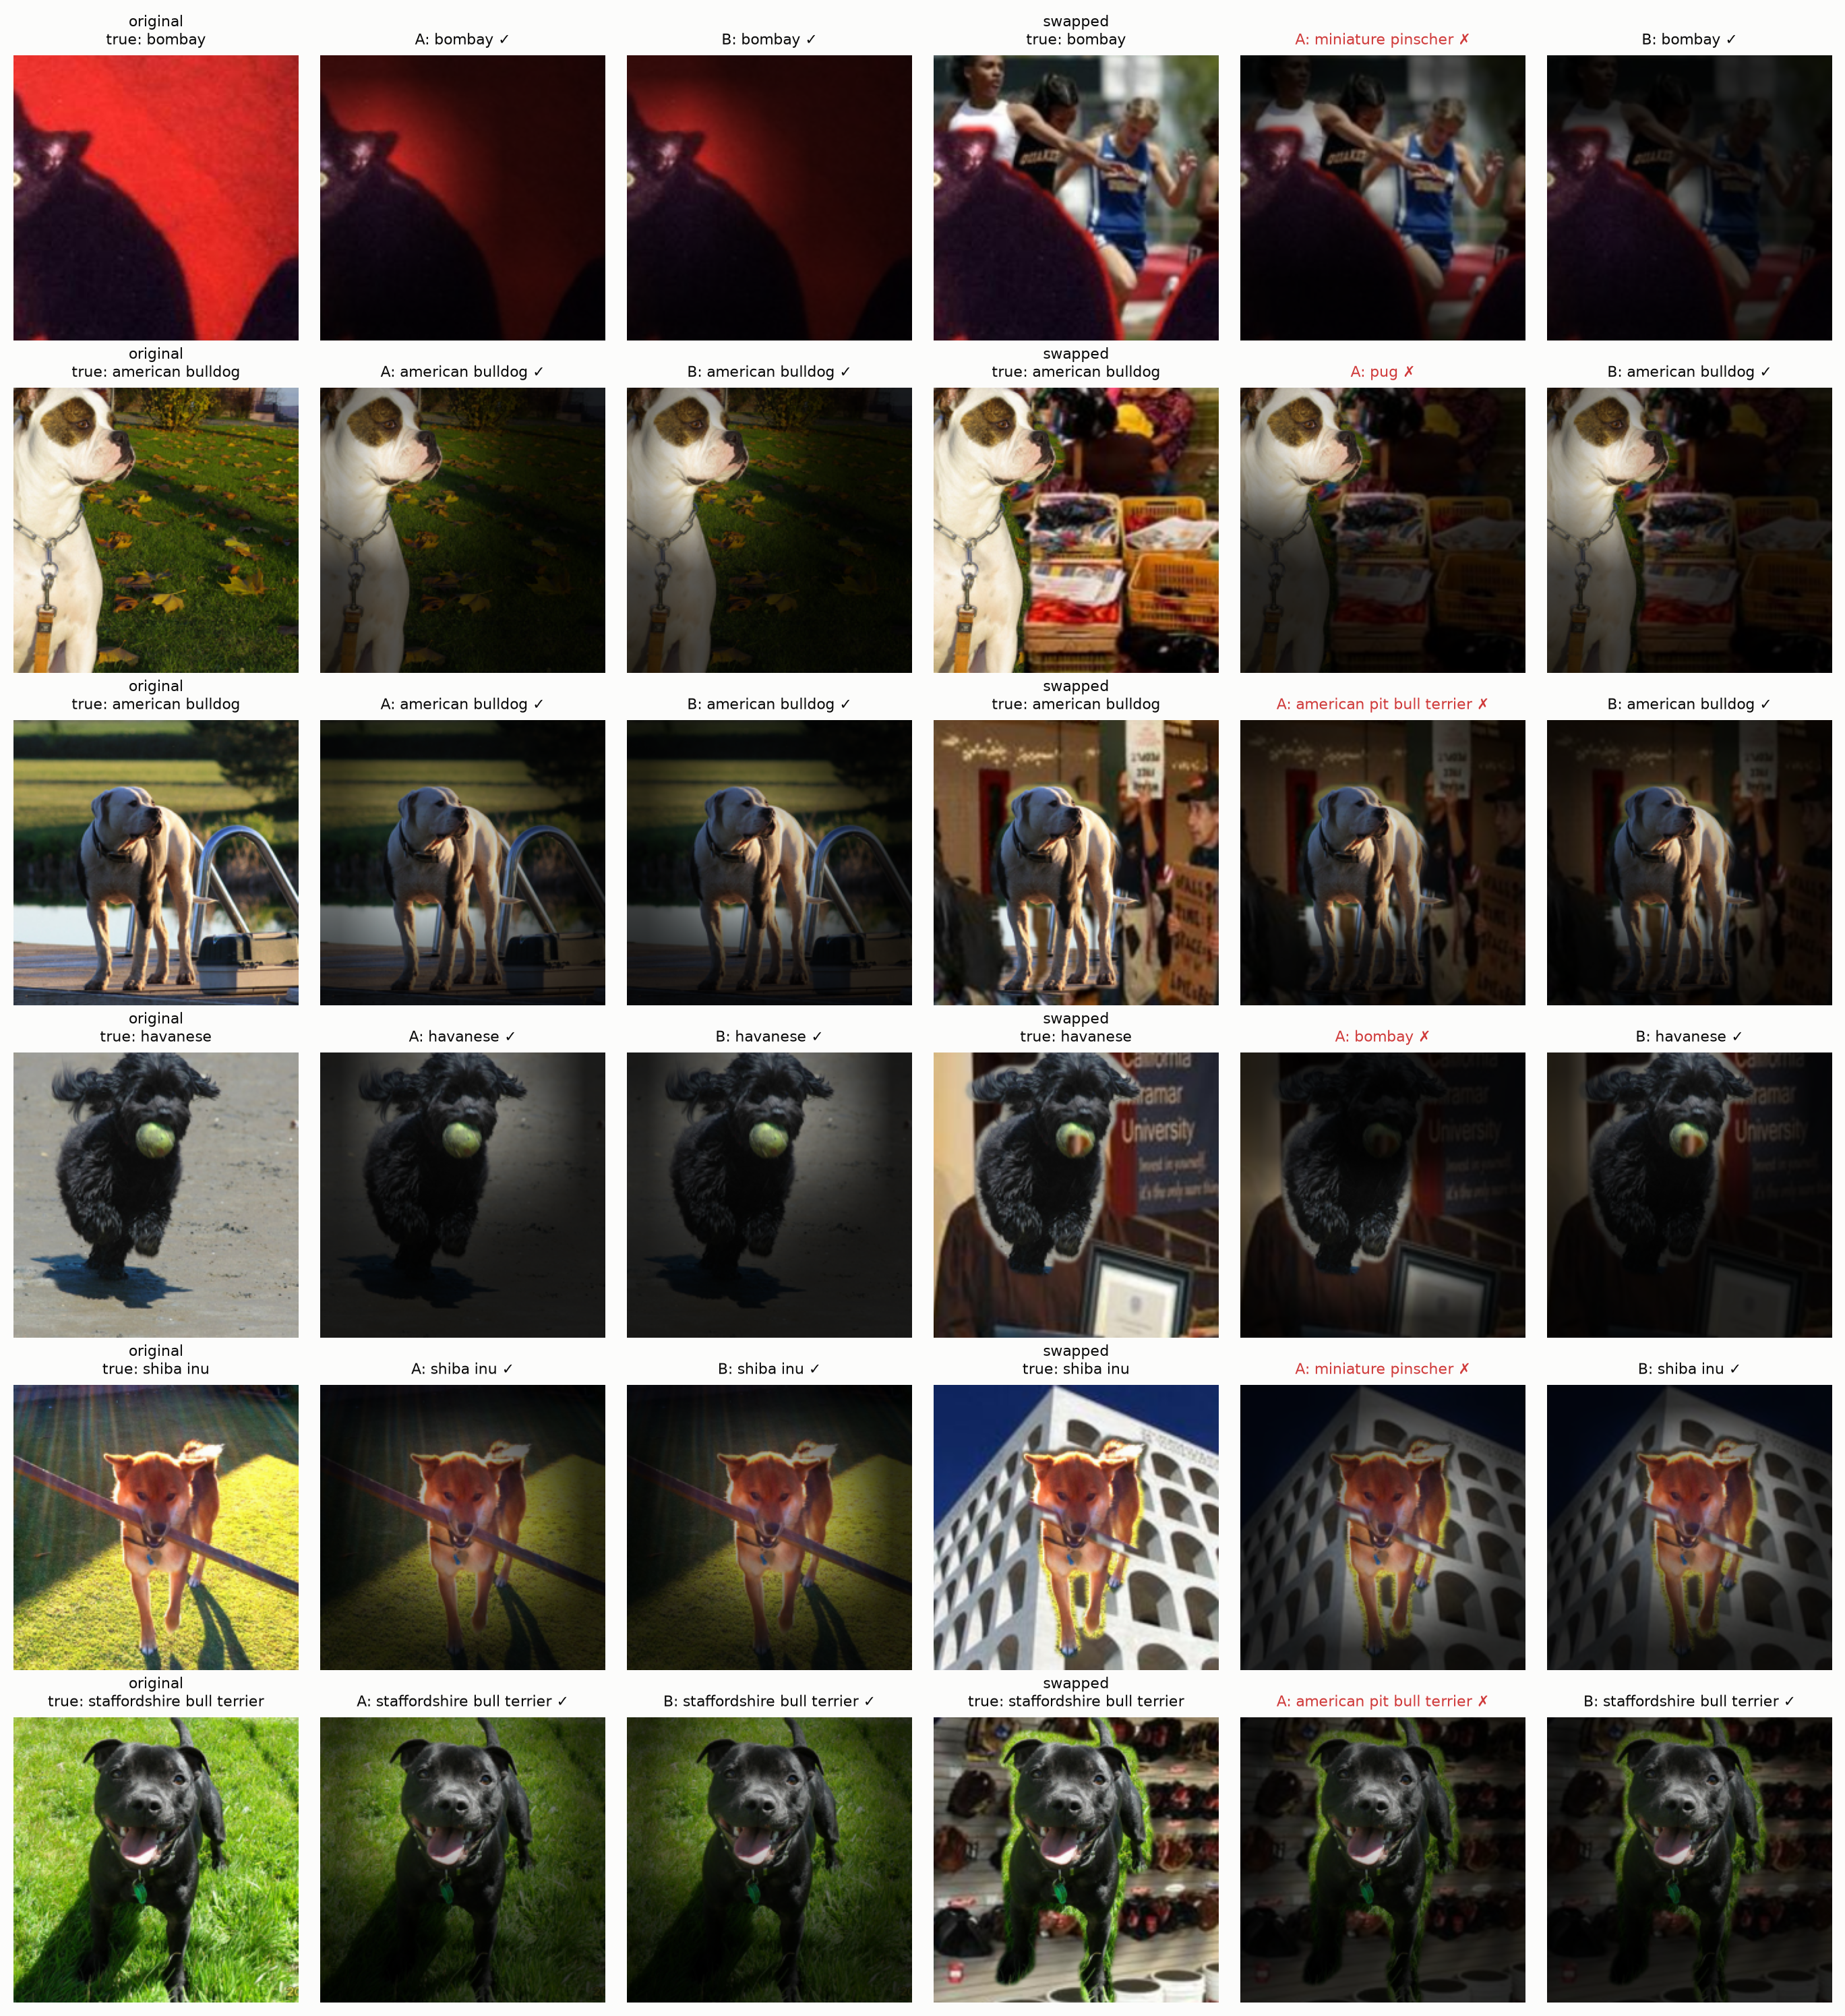
\includegraphics[width=\textwidth]{fig4_flip_examples_gradcam}
\caption{Images that every seed of A gets right on the original and wrong on the swapped version, while every seed of
B gets both right. Columns: original image, Grad-CAM of A, Grad-CAM of B, swapped image, Grad-CAM of A (red = wrong
prediction), Grad-CAM of B. Typical confusions: Staffordshire $\to$ pit bull, American bulldog $\to$ pug / pit bull.}
\label{fig:gradcam}
\end{figure}
All models put about $77$--$80\%$ of their Grad-CAM mass on the pet, well above its $59\%$ area, and A and B do not
differ (Table~\ref{tab:gradcam}). So Grad-CAM does not show the difference that accuracy, flip rate and probing show.
This is a known limitation of Grad-CAM: it is coarse ($7\times7$), it explains only the predicted class, and a model
can look mostly at the pet while a small amount of background context still changes the decision on ambiguous images.
Figure~\ref{fig:gradcam} shows such flips.

\subsection{What do the features know about the background? Probing}
\begin{table}[h]
\centering\small
\begin{subtable}{0.58\textwidth}\centering
\begin{adjustbox}{max width=\linewidth}
\begin{tabular}{lccc}
\toprule
Architecture & Before fine-tuning & A & B \\
\midrule
\tableinput tables/probing_arch.tex 
\bottomrule
\end{tabular}
\end{adjustbox}
\caption{Architectures}
\end{subtable}\hfill
\begin{subtable}{0.4\textwidth}\centering
\begin{adjustbox}{max width=\linewidth}
\begin{tabular}{lc}
\toprule
ResNet-18 variant & Scene acc. (\%) \\
\midrule
\tableinput tables/probing_methods.tex 
\bottomrule
\end{tabular}
\end{adjustbox}
\caption{Training strategies}
\end{subtable}
\caption{Linear-probe accuracy (\%) for the background scene category (87 classes, chance 1.1\%), on penultimate
features of swapped test images; 5-fold CV, mean $\pm$ std over seeds.}
\label{tab:probing}
\end{table}
\begin{figure}[h]
\centering
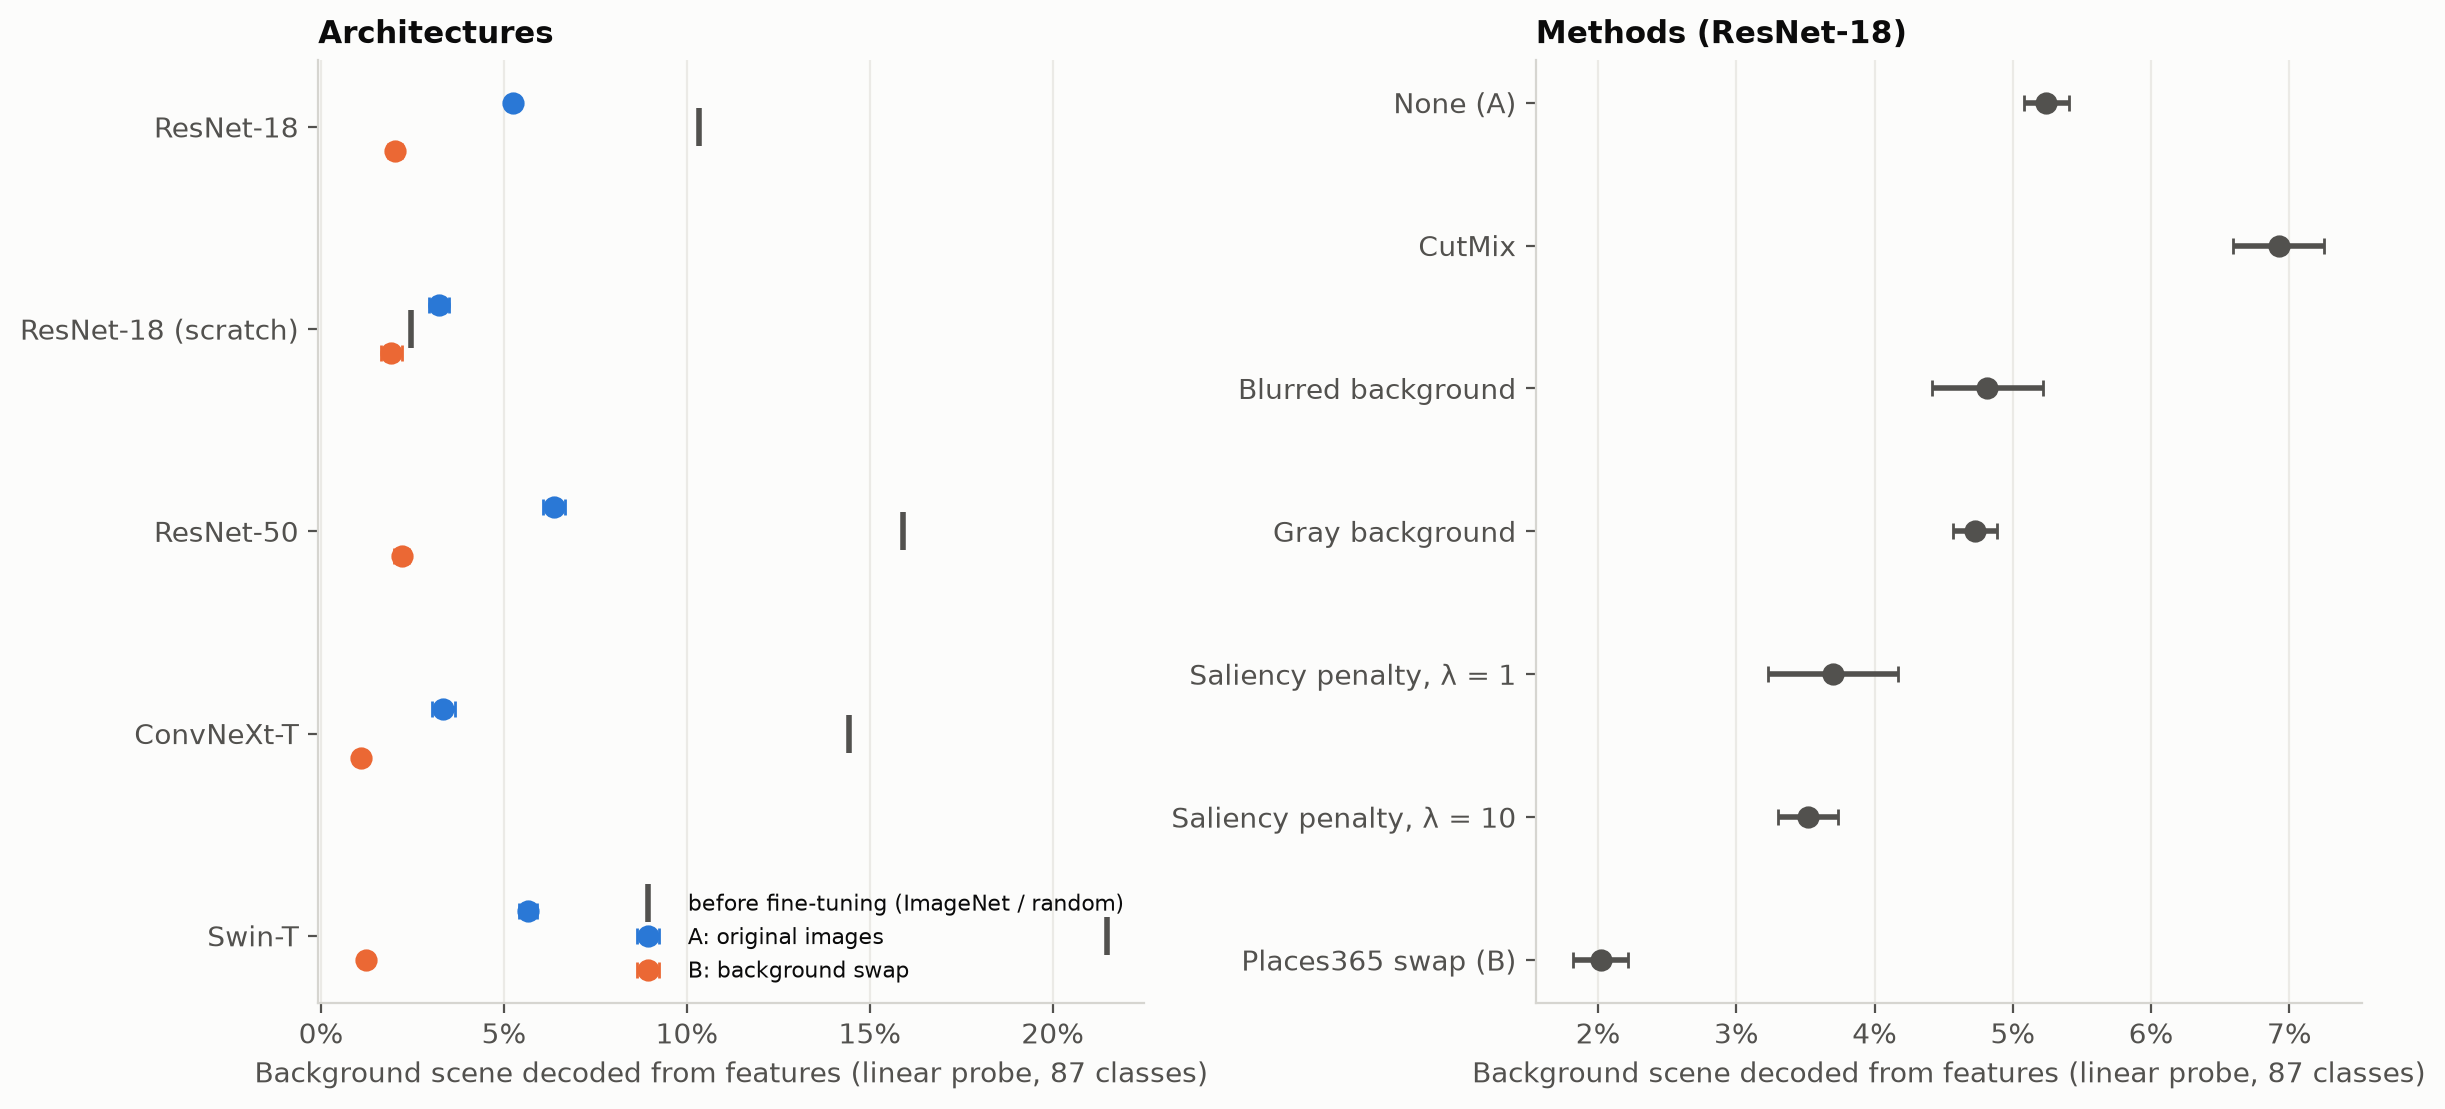
\includegraphics[width=\textwidth]{fig7_probing}
\caption{Background-scene probe accuracy per model.}
\label{fig:probing}
\end{figure}
ImageNet features encode the scene well ($10$--$21\%$, i.e.\ $9$--$19\times$ chance), which is expected: recognising
scenes is useful for ImageNet. Fine-tuning on pets removes much of it (A: $3$--$6\%$), and background swapping removes
most of the rest (B: $1.1$--$2.2\%$, close to chance; Table~\ref{tab:probing}). Among the training strategies, every one that leaves a sizeable gap (gray, blur, CutMix, saliency penalty) also
leaves $3.5$--$6.9\%$ scene accuracy, while the random swap with $p\ge0.25$ leaves $1.9$--$2.8\%$; CutMix, the
strategy with the largest gap, also has the most scene information ($6.9\%$). This is the mechanism behind
H2: B learns features that are \emph{invariant} to the background, so a new scene does not move them.

\subsection{Transfer to real photos: Stanford Dogs}
\begin{table}[h]
\centering\small
\setlength{\tabcolsep}{4pt}
\begin{adjustbox}{max width=\linewidth}
\begin{tabular}{lccccc}
\toprule
Model & Full photo (\%) & Dog crop (\%) & Full, dogs only (\%) & Pet test (\%) & B$-$A full [95\% CI] (p.p.) \\
\midrule
\tableinput tables/stanford_dogs.tex 
\bottomrule
\end{tabular}
\end{adjustbox}
\caption{External test: 3{,}730 Stanford Dogs photos of 21 Pet breeds, 37-way prediction (``dogs only'' = argmax over
the 21 breeds). The last column is a paired bootstrap over photos against the corresponding A model (for the
strategies: against ResNet-18 A).}
\label{tab:sd}
\end{table}
\begin{figure}[h]
\centering
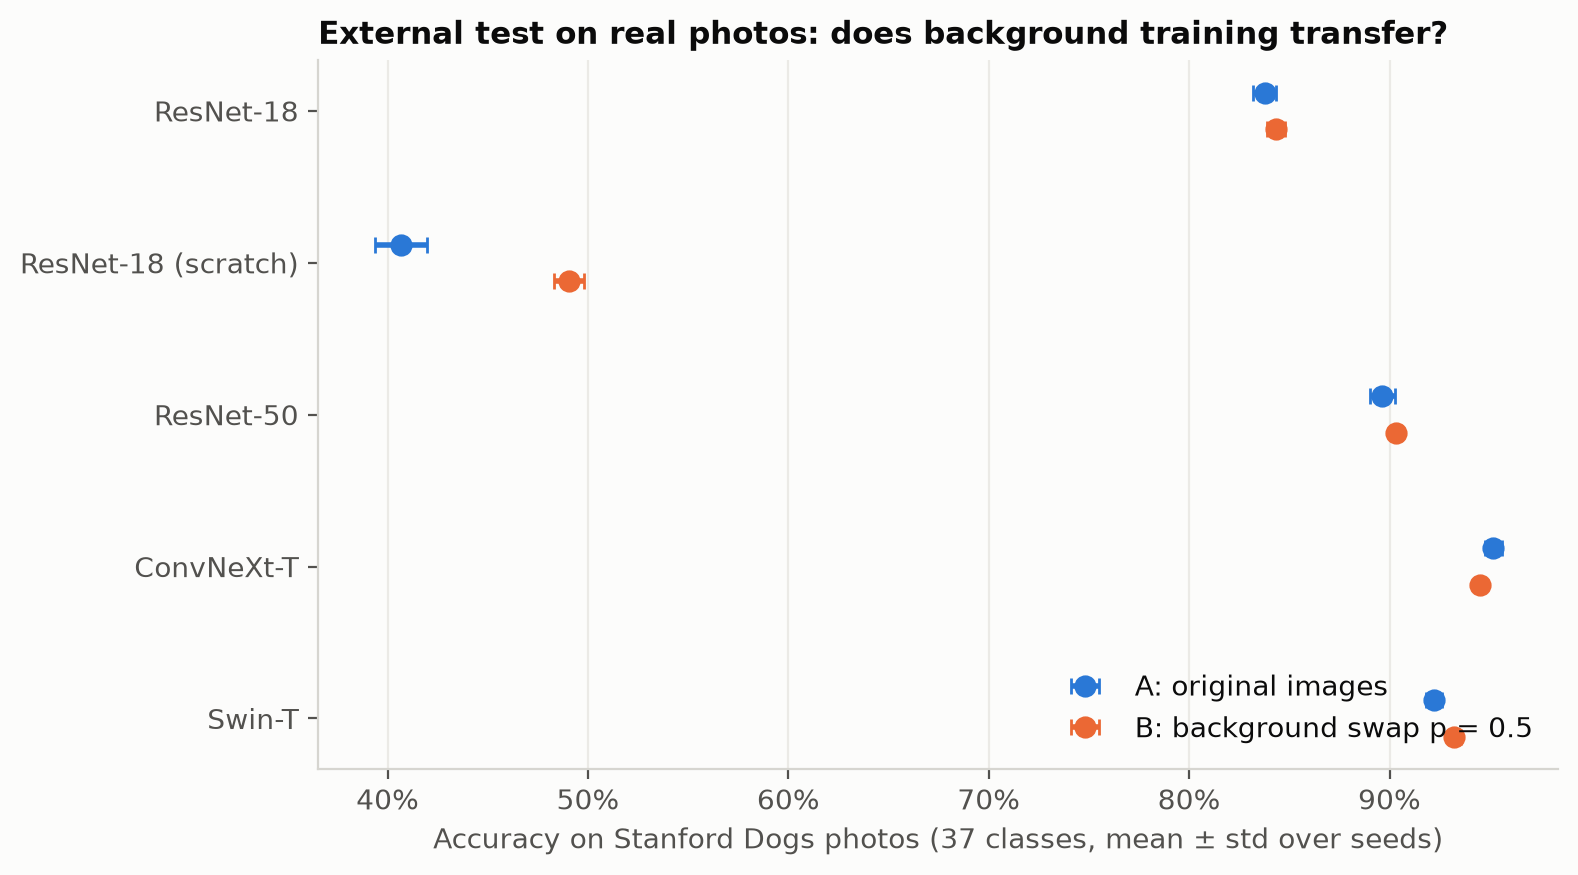
\includegraphics[width=0.75\textwidth]{fig8_stanford_dogs}
\caption{Stanford Dogs accuracy (full photos) of A and B for each architecture.}
\label{fig:sd}
\end{figure}
On real photos with natural backgrounds, B is at least as good as A for four of five architectures and significantly
better for ResNet-50 ($+0.7$\pp), Swin-T ($+1.0$\pp) and the scratch model ($+8.4$\pp); for ResNet-18 the gain is
$+0.5$\pp{} with a CI that touches 0 (Table~\ref{tab:sd}, Fig.~\ref{fig:sd}). ConvNeXt-T is the exception ($-0.7$\pp, CI
excludes 0), at the highest accuracy of all ($95\%$). All alternative strategies are equal to or worse than A here,
and the saliency penalty with $\lambda=10$ loses $7.7$\pp. So the swap does not just teach the model to handle our
composites; it does not hurt, and mostly helps, on a natural distribution shift. Cropping to the dog box lowers
accuracy for all models (e.g.\ ResNet-18 A $83.8\to69.6\%$). The likely reason is that many crops are small and are
upscaled to 224 px, and that tight boxes cut off parts of the body and change the framing the networks were trained on,
so this view is harder rather than ``cleaner''; the A--B ordering on crops is the same as on full photos.

\subsection{Case study: Waterbirds}\label{sec:waterbirds}
\begin{table}[h]
\centering\small
\setlength{\tabcolsep}{4pt}
\begin{adjustbox}{max width=\linewidth}
\begin{tabular}{lcccccc}
\toprule
Model (ResNet-18) & Average & Worst group & Landbird/land & Landbird/water & Waterbird/land & Waterbird/water \\
\midrule
\tableinput tables/waterbirds.tex 
\bottomrule
\end{tabular}
\end{adjustbox}
\caption{Waterbirds test accuracy (\%), mean $\pm$ std over 3 seeds. The worst group is waterbird on land for every
run.}
\label{tab:wb}
\end{table}
\begin{figure}[h]
\centering
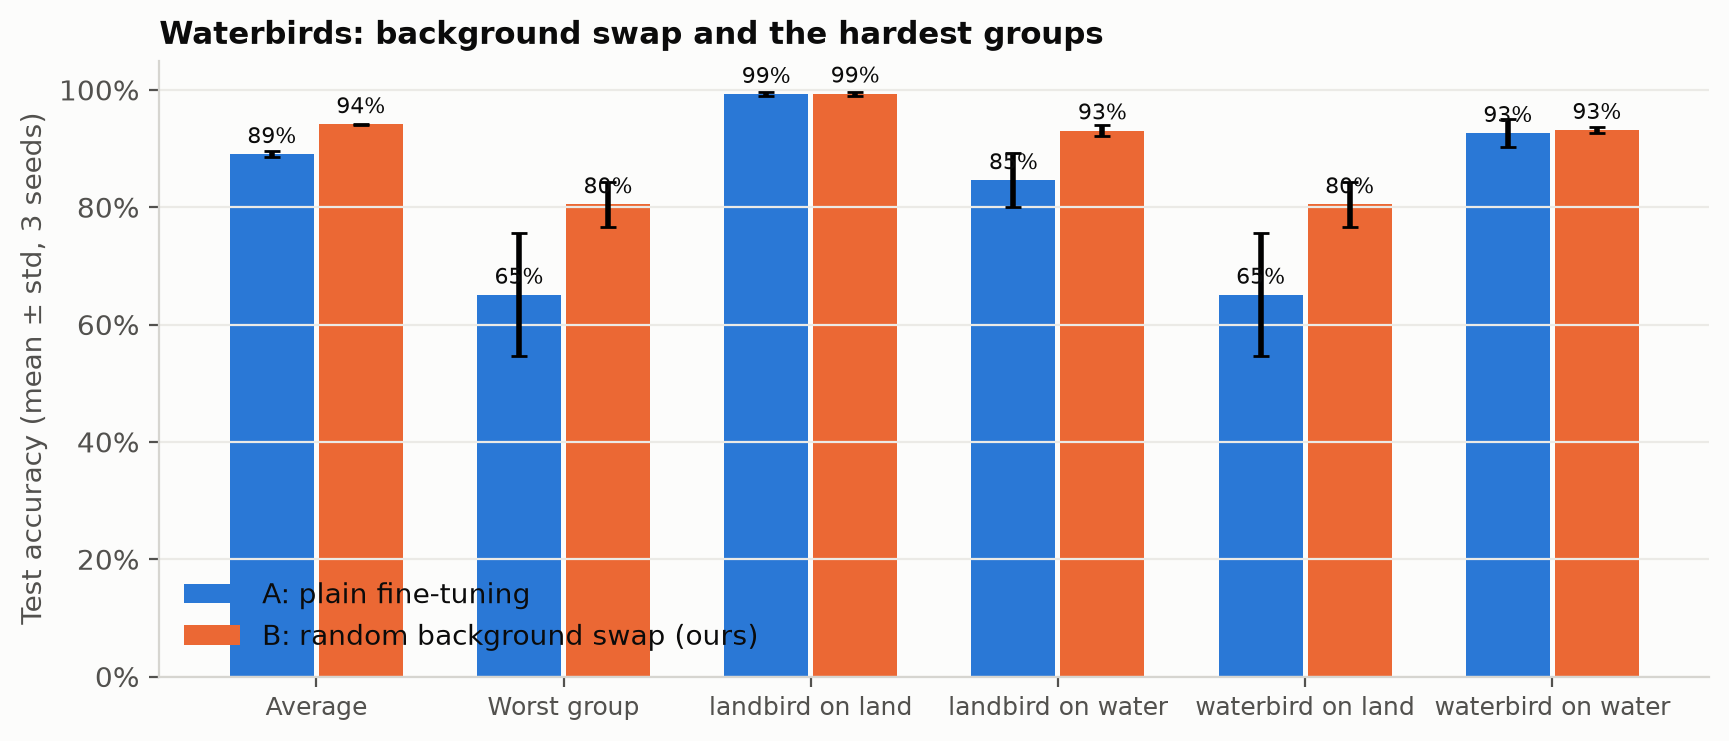
\includegraphics[width=0.85\textwidth]{fig9_waterbirds}
\caption{Waterbirds: average accuracy, worst-group accuracy and per-group accuracy of A and B.}
\label{fig:wb}
\end{figure}
Here the background is a real shortcut: it predicts the label 95\% of the time in training. Plain fine-tuning reaches
$89.0\%$ on average but only $65.1\pm10.5\%$ on waterbirds photographed on land. The same swap remedy, unchanged
(random scenes from our Places365 train pool, $p=0.5$, automatic DeepLabV3 masks, no group labels), raises the
worst-group accuracy to $80.5\pm3.9\%$ ($+15$\pp), the average accuracy to $94.1\%$, and the landbird-on-water group
from $84.6$ to $93.1\%$, while the majority groups stay at $93$--$99\%$ (Table~\ref{tab:wb}, Fig.~\ref{fig:wb}). It also
makes training far more stable: the worst-group std falls from $10.5$ to $3.9$\pp.

\subsection{Validation versus test}
Validation accuracies (Table~\ref{tab:training}) are 2.5--4\pp{} higher than test accuracies for the pretrained
models (e.g.\ ResNet-18 A $92.9\%$ vs $89.7\%$) and 6--10\pp{} for the scratch models. Two reasons: the checkpoint was \emph{selected} on validation (selection bias),
and the validation set is small (552 images, $\pm1.1$\pp{} binomial standard error). The ranking of models and the
A/B gaps are the same on validation and test, which is the evidence that the test results are not a fluke of one split.

%======================================================================
\section{Discussion}\label{sec:discussion}
%======================================================================

\paragraph{Distraction, not a breed--background shortcut (on Pet).} Two observations together lead to this reading.
(1) The bg-only accuracy of ResNet-18 is near chance, so the background alone says almost nothing about the breed to
this model. (2) Yet swapping the background changes $8.4\%$ of A's predictions. A model that ignored the background
would change none; a model that used a breed--background association would also do well on bg-only. The consistent
picture is that A's features mix pet and scene, and an unfamiliar scene shifts the features enough to push ambiguous
images (Staffordshire vs pit bull) across a decision boundary. Probing supports this: A's features still encode the
scene, B's mostly do not.

\paragraph{Why random scenes work and gray/blur do not fully.} Gray and blur teach invariance to the \emph{absence} of
a background. The swapped test asks for invariance to the \emph{presence of a wrong} background. Only random scenes
provide training examples of that, and in thousands of variations (209 categories, a new draw every epoch). In
probabilistic terms, the swap makes the background statistically independent of the label in the training
distribution; the other strategies only weaken the dependence.

\paragraph{Why the saliency penalty fails here.} RRR controls the first-order sensitivity
$\partial p/\partial x$ around training images. A background swap is not a small perturbation: it replaces about 60\% of
the pixels. A model can be locally flat on the background and still respond strongly to a completely different scene.
It also competes with the classification loss: at $\lambda=10$ the model gives up $5$\pp{} of accuracy and becomes
\emph{less} robust.

\paragraph{Why bg-only is above chance for strong models.} Bg-only images keep the shape of the pet as a gray
silhouette. Ears, tail and body proportions are informative for breed (e.g.\ Basset hound vs Pomeranian). A
strong model can recognise some breeds from the silhouette alone. B does not lower bg-only for ConvNeXt-T
($9.6\to9.2\%$), which is what we expect if the information is shape, since swapping preserves the shape. A
silhouette-free control (e.g.\ inpainting the pet region) would separate shape from context; we leave it to future work.

\paragraph{Is there a price?} On original images, no: B matches A within the seed spread for every pretrained
architecture, and improves the scratch model. Costs are elsewhere: training needs foreground masks (available here,
produced automatically by a segmentation network for Waterbirds) and about 35\% more time per epoch for compositing
(ResNet-18: 5.1 vs 6.9 min per run, Table~\ref{tab:training}).

\paragraph{ConvNeXt on Stanford Dogs.} It is the only significant negative transfer result ($-0.7$\pp). Its A model is
already the least background-sensitive on Pet (gap $1.0$\pp) and the most accurate on Stanford Dogs ($95.2\%$), and
Stanford Dogs photos were part of its ImageNet pretraining data. One plausible explanation is that B moves ConvNeXt
slightly further from its pretrained solution, which is especially good on exactly these photos. We report it as an
honest exception.

%======================================================================
\section{Limitations}
%======================================================================
\begin{itemize}
  \item \textbf{Synthetic shift.} Swapped images are composites; despite soft masks they can show seams and lighting
  mismatch. We control for this with fg-only and check transfer on real photos, but a composite is not a real photo of
  a pet in that scene.
  \item \textbf{Masks.} Trimaps are human annotations with an uncertain border, which we assign to the pet; a few masks
  are almost empty. On Waterbirds, DeepLabV3 masks are imperfect (images with a mask below 0.5\% of the area are left
  unswapped).
  \item \textbf{Silhouette leakage} in bg-only (see Discussion).
  \item \textbf{Hyperparameters} were tuned for ResNet-18 A and reused for all models; each architecture might do
  better with its own recipe. HOG's best $C$ lies at the edge of the grid, so the baseline may be slightly
  under-tuned (it is not central to any claim).
  \item \textbf{Three seeds} give a rough estimate of training variance; std over 3 values is itself noisy. Bootstrap
  intervals cover test-set sampling, not training randomness.
  \item \textbf{ImageNet overlap} with Stanford Dogs inflates absolute external accuracies (but not the A--B comparison).
  \item \textbf{Scope.} One dataset family per question, one remedy family; no comparison with group-DRO or
  last-layer retraining on Waterbirds.
\end{itemize}

%======================================================================
\section{Conclusion}
%======================================================================
A standard fine-tuned ResNet-18 that classifies pet breeds with $89.7\%$ accuracy changes $8.4\%$ of its answers
when only the background is replaced. It does not read the breed off the background; it is distracted by unfamiliar
scenes, and for near-identical breeds that is enough to flip the decision. Replacing the background of training
images by random scenes, already for a quarter of them, removes this sensitivity for every architecture we tried,
costs no accuracy, strips background information out of the learned features, and works better than gray or blurred
backgrounds, CutMix or a saliency penalty. The same simple fix transfers to real photographs and raises worst-group
accuracy on the Waterbirds shortcut benchmark from $65\%$ to $80\%$. The broader lesson for shortcut learning: test
accuracy alone hides the problem; you have to break the correlation on purpose to see it, and if you can separate
object from context (with masks or a segmentation model), randomising the context is a cheap and effective remedy.

\paragraph{Reproducibility and compute.} Code, configs, splits, background manifests, per-image predictions of every
run, training histories and the scripts that build every table and figure are in the repository. Every notebook runs
end-to-end in Google Colab (``Run all''). The final set of 51 Pet runs and 6 Waterbirds runs was trained on a single
local NVIDIA GPU; per-run times are in Table~\ref{tab:training} (5--10 min for pretrained models, 14--18 min for
scratch models). Checkpoints ($\approx$13.5\,GB) are stored outside git.

% TODO (team): check and edit the contributions before submission.
\paragraph{Team contributions.} Amina Abdikalyk: project plan, splits, evaluation protocol, analysis, report.
Islam Sanatbek: data pipeline, masks, background pools and compositing. Tomiris Rakymbay: HOG + SVM baseline,
evaluation metrics, error analysis. Assylkhan Tleubayev: training pipeline, model training, Grad-CAM.

%======================================================================
\begin{thebibliography}{99}\small
\bibitem{alain2016probes} G.~Alain and Y.~Bengio. Understanding intermediate layers using linear classifier probes. \emph{arXiv:1610.01644}, 2016.
\bibitem{beery2018terra} S.~Beery, G.~Van~Horn, and P.~Perona. Recognition in terra incognita. In \emph{ECCV}, 2018.
\bibitem{chen2017deeplab} L.-C.~Chen, G.~Papandreou, F.~Schroff, and H.~Adam. Rethinking atrous convolution for semantic image segmentation. \emph{arXiv:1706.05587}, 2017.
\bibitem{dalal2005hog} N.~Dalal and B.~Triggs. Histograms of oriented gradients for human detection. In \emph{CVPR}, 2005.
\bibitem{deng2009imagenet} J.~Deng, W.~Dong, R.~Socher, L.-J.~Li, K.~Li, and L.~Fei-Fei. ImageNet: A large-scale hierarchical image database. In \emph{CVPR}, 2009.
\bibitem{efron1993bootstrap} B.~Efron and R.~J.~Tibshirani. \emph{An Introduction to the Bootstrap}. Chapman \& Hall, 1993.
\bibitem{geirhos2020shortcut} R.~Geirhos, J.-H.~Jacobsen, C.~Michaelis, R.~Zemel, W.~Brendel, M.~Bethge, and F.~A.~Wichmann. Shortcut learning in deep neural networks. \emph{Nature Machine Intelligence}, 2(11):665--673, 2020.
\bibitem{he2016resnet} K.~He, X.~Zhang, S.~Ren, and J.~Sun. Deep residual learning for image recognition. In \emph{CVPR}, 2016.
\bibitem{khosla2011dogs} A.~Khosla, N.~Jayadevaprakash, B.~Yao, and L.~Fei-Fei. Novel dataset for fine-grained image categorization: Stanford Dogs. In \emph{CVPR Workshop on Fine-Grained Visual Categorization}, 2011.
\bibitem{liu2021swin} Z.~Liu, Y.~Lin, Y.~Cao, H.~Hu, Y.~Wei, Z.~Zhang, S.~Lin, and B.~Guo. Swin Transformer: Hierarchical vision transformer using shifted windows. In \emph{ICCV}, 2021.
\bibitem{liu2022convnext} Z.~Liu, H.~Mao, C.-Y.~Wu, C.~Feichtenhofer, T.~Darrell, and S.~Xie. A ConvNet for the 2020s. In \emph{CVPR}, 2022.
\bibitem{loshchilov2017sgdr} I.~Loshchilov and F.~Hutter. SGDR: Stochastic gradient descent with warm restarts. In \emph{ICLR}, 2017.
\bibitem{loshchilov2019adamw} I.~Loshchilov and F.~Hutter. Decoupled weight decay regularization. In \emph{ICLR}, 2019.
\bibitem{parkhi2012cats} O.~M.~Parkhi, A.~Vedaldi, A.~Zisserman, and C.~V.~Jawahar. Cats and dogs. In \emph{CVPR}, 2012.
\bibitem{ribeiro2016lime} M.~T.~Ribeiro, S.~Singh, and C.~Guestrin. ``Why should I trust you?'' Explaining the predictions of any classifier. In \emph{KDD}, 2016.
\bibitem{ross2017rrr} A.~S.~Ross, M.~C.~Hughes, and F.~Doshi-Velez. Right for the right reasons: Training differentiable models by constraining their explanations. In \emph{IJCAI}, 2017.
\bibitem{sagawa2020dro} S.~Sagawa, P.~W.~Koh, T.~B.~Hashimoto, and P.~Liang. Distributionally robust neural networks for group shifts. In \emph{ICLR}, 2020.
\bibitem{selvaraju2017gradcam} R.~R.~Selvaraju, M.~Cogswell, A.~Das, R.~Vedantam, D.~Parikh, and D.~Batra. Grad-CAM: Visual explanations from deep networks via gradient-based localization. In \emph{ICCV}, 2017.
\bibitem{wah2011cub} C.~Wah, S.~Branson, P.~Welinder, P.~Perona, and S.~Belongie. The Caltech-UCSD Birds-200-2011 dataset. Technical report CNS-TR-2011-001, Caltech, 2011.
\bibitem{xiao2021noise} K.~Xiao, L.~Engstrom, A.~Ilyas, and A.~Madry. Noise or signal: The role of image backgrounds in object recognition. In \emph{ICLR}, 2021.
\bibitem{yun2019cutmix} S.~Yun, D.~Han, S.~J.~Oh, S.~Chun, J.~Choe, and Y.~Yoo. CutMix: Regularization strategy to train strong classifiers with localizable features. In \emph{ICCV}, 2019.
\bibitem{zech2018pneumonia} J.~R.~Zech, M.~A.~Badgeley, M.~Liu, A.~B.~Costa, J.~J.~Titano, and E.~K.~Oermann. Variable generalization performance of a deep learning model to detect pneumonia in chest radiographs: A cross-sectional study. \emph{PLOS Medicine}, 15(11):e1002683, 2018.
\bibitem{zhou2018places} B.~Zhou, A.~Lapedriza, A.~Khosla, A.~Oliva, and A.~Torralba. Places: A 10 million image database for scene recognition. \emph{IEEE TPAMI}, 40(6):1452--1464, 2018.
\end{thebibliography}

%======================================================================
\appendix
\section{Additional tables and figures}
%======================================================================

\begin{table}[h]
\centering\small
\begin{adjustbox}{max width=\linewidth}
\begin{tabular}{lcccc}
\toprule
Model & Original & Swapped & Fg-only & Bg-only \\
\midrule
\tableinput tables/f1_all.tex 
\bottomrule
\end{tabular}
\end{adjustbox}
\caption{Macro F1 (\%) on the Pet test set, mean $\pm$ std over seeds.}
\label{tab:f1}
\end{table}

\begin{table}[h]
\centering\small
\setlength{\tabcolsep}{4pt}
\begin{adjustbox}{max width=\linewidth}
\begin{tabular}{lcccccc}
\toprule
Model & Epochs & Best epoch per seed & Val. original (\%) & Val. swapped (\%) & Final train acc. (\%) & Min / run \\
\midrule
\tableinput tables/training.tex 
\bottomrule
\end{tabular}
\end{adjustbox}
\caption{Training summary. ``Best epoch'' is the selected checkpoint (1-based) for seeds 0, 1, 2; validation accuracies
are those of the selected checkpoint. Train accuracy of CutMix is measured on mixed images against the hard label and is
therefore lower.}
\label{tab:training}
\end{table}

\begin{table}[h]
\centering\small
\begin{adjustbox}{max width=\linewidth}
\begin{tabular}{lcrrrrrr}
\toprule
Model & Seed & Average & Worst group & L/land & L/water & W/land & W/water \\
\midrule
\tableinput tables/waterbirds_per_seed.tex 
\bottomrule
\end{tabular}
\end{adjustbox}
\caption{Waterbirds test accuracy (\%) per seed (L = landbird, W = waterbird).}
\end{table}

{\small
\setlength{\tabcolsep}{5pt}
\begin{longtable}{lcrrrrrr}
\caption{Every Pet run on the test set (\%). Gap in \pp.}\label{tab:perrun}\\
\toprule
Model & Seed & Original & Swapped & Fg-only & Bg-only & Gap swap & Flip \\
\midrule
\endfirsthead
\toprule
Model & Seed & Original & Swapped & Fg-only & Bg-only & Gap swap & Flip \\
\midrule
\endhead
\bottomrule
\endfoot
\tableinput tables/per_run.tex 
\end{longtable}
}

\begin{figure}[p]
\centering
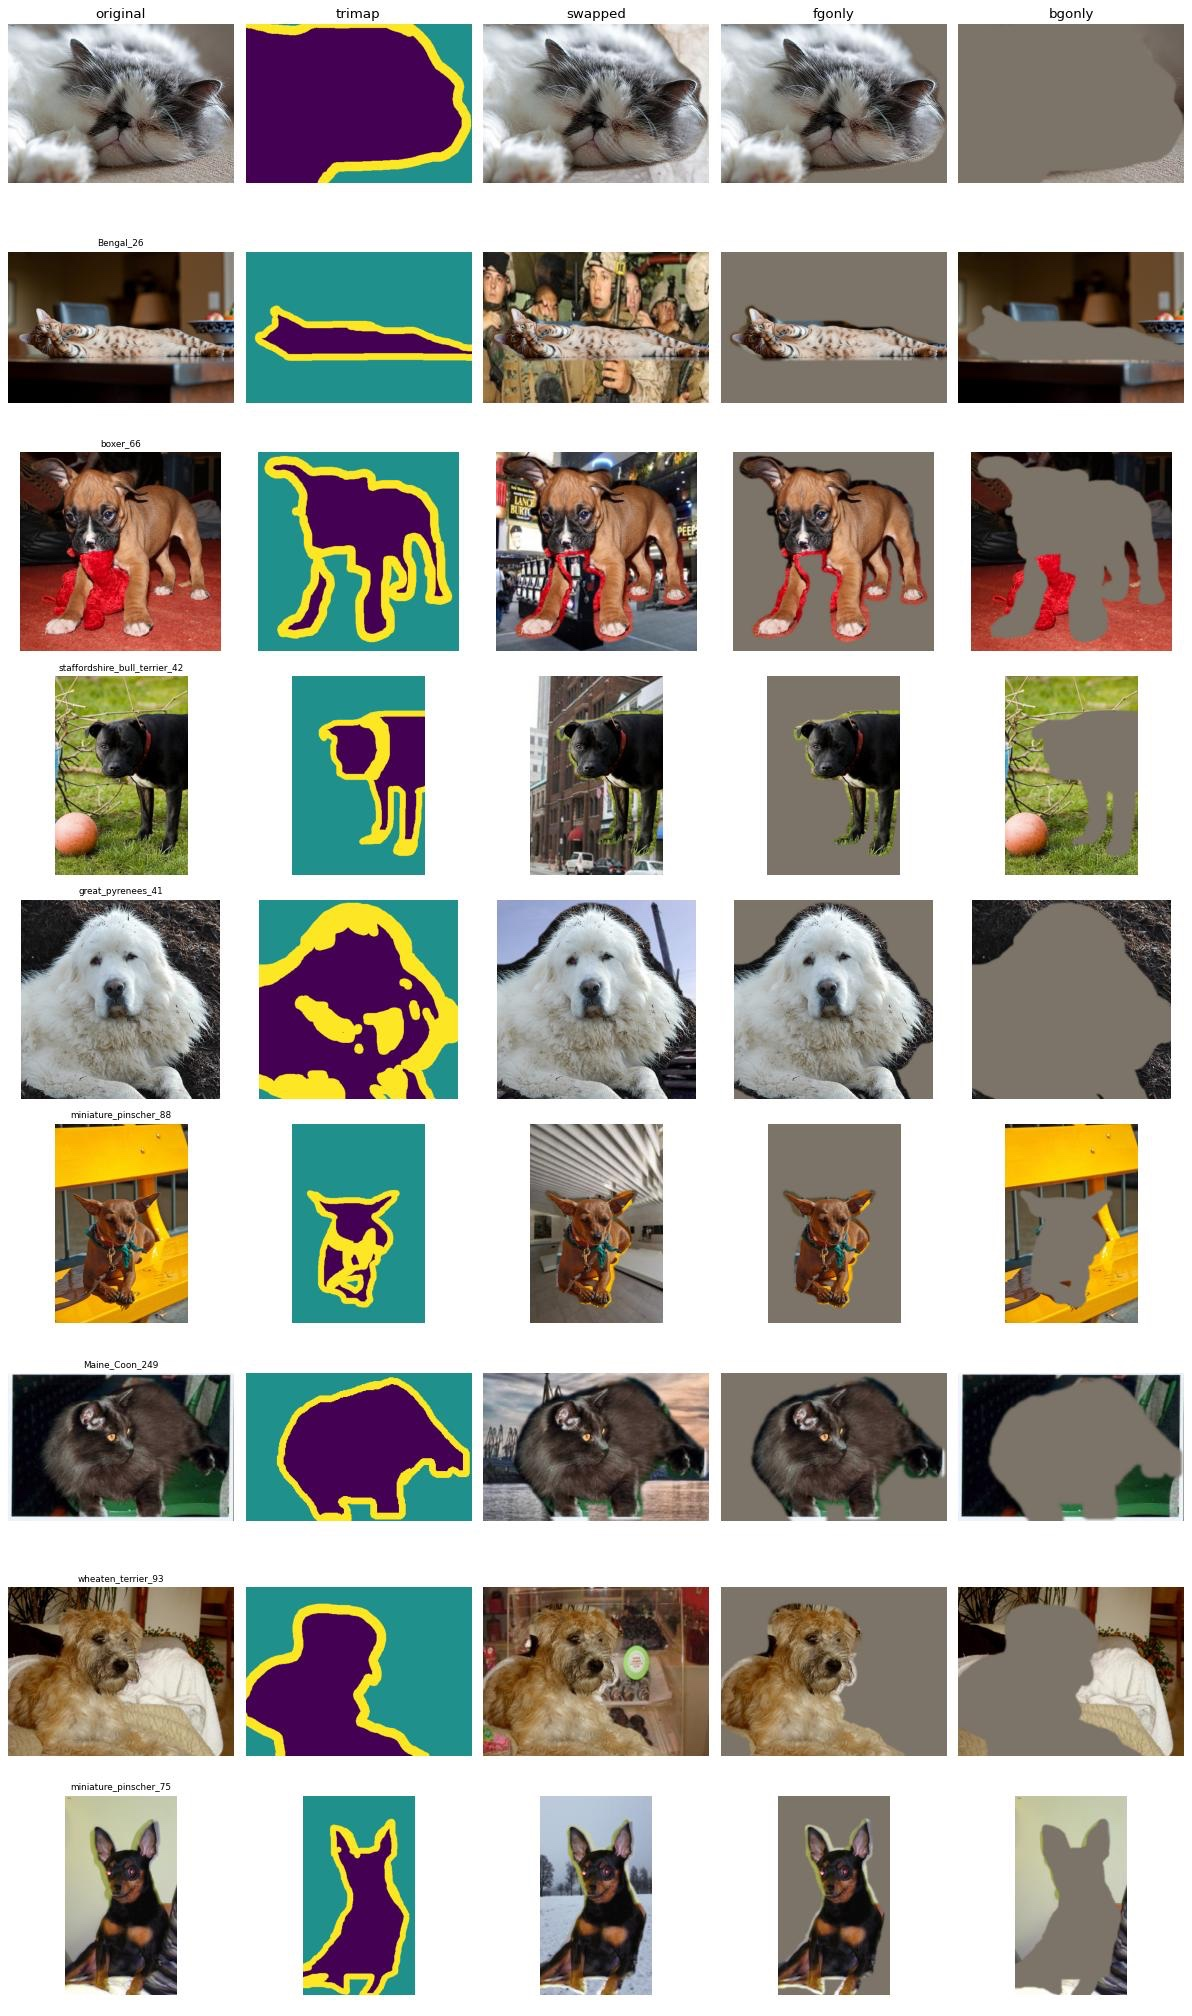
\includegraphics[width=0.8\textwidth]{week1_gallery_top}
\caption{Examples from the data pipeline (first rows of the gallery made in week 1). Columns: original image, trimap
(purple = pet, yellow = border, teal = background), pet on a new Places365 background (swapped), pet on the neutral
gray background (fg-only), pet painted over with gray (bg-only).}
\label{fig:gallery}
\end{figure}

%======================================================================
\section{Anticipated questions}
%======================================================================
\begin{description}[style=nextline,leftmargin=0pt]
\item[Why not just evaluate on more test data instead of making composites?]
Ordinary test data has the same background statistics as training data, so a background shortcut is invisible there.
Composites let us change \emph{only} the background and keep the pet pixel-identical, which turns a vague question
(``does it use the background?'') into a measurable difference between two inputs.

\item[Are the swapped test backgrounds really unseen?]
Yes, at two levels. The three background pools share no image, and they share no \emph{scene category}: the 87 test
categories never appear in training (Table~\ref{tab:pools}).

\item[Could the gap come from paste artifacts and not from the background?]
That is what fg-only controls. Fg-only images have the same seams and the same blending but a neutral background.
A drops $1.1$\pp{} there vs $2.8$\pp{} on swapped images, so most of the drop is due to the scene. Also, B was trained
with composites and might simply have learned to ignore seams; but B's fg-only gain over A ($+0.8$\pp) is smaller than
its swapped gain ($+2.2$\pp), and B also helps on real Stanford Dogs photos, which have no seams.

\item[Isn't B just seeing more data / more augmentation?]
B sees the same images for the same number of steps; only the background of half of them is replaced. CutMix,
gray and blur are also extra augmentations at the same rate, and none of them removes the gap. So it is the specific
content of the augmentation, a random but realistic background, that matters.

\item[Why choose the checkpoint on original validation accuracy?]
To be fair to A. If we selected by swapped validation accuracy we would be optimising robustness on purpose, which
would favour B. With selection on original images, both models are chosen for what the user would normally optimise.

\item[Why $p=0.5$ for B, if $p=0.25$ already works?]
$p=0.5$ was fixed before the ablation as the natural midpoint. The ablation then showed that the result is not
sensitive to $p$ in $[0.25,0.5]$, and that $p=1$ starts to cost original accuracy.

\item[Why is the flip rate larger than the gap?]
The gap is a net change (wrong$\to$right cancels right$\to$wrong); the flip rate counts every change, including changes
between two wrong classes. $\flip\ge|\gap|$ always.

\item[How significant is the A vs B difference?]
Across 3 seeds the gaps are $2.8\pm0.7$ vs $0.5\pm0.2$\pp. Across test images the paired bootstrap gives
\bootDiff\pp, 95\% CI [\bootLo, \bootHi], with no bootstrap sample $\le0$. For every architecture the CI excludes 0
(Table~\ref{tab:arch}).

\item[Why is bg-only accuracy near chance, but the gap still positive?]
Because the model does not need the background to carry breed information to be disturbed by it. A new scene shifts
the feature vector; for images near the boundary between two similar breeds, a small shift changes the decision. The
per-breed results (Staffordshire vs pit bull) show exactly this.

\item[Why does Grad-CAM not show a difference between A and B?]
Grad-CAM has $7\times7$ resolution, explains one class, and measures where the gradient of the chosen class is large,
not how much the decision would change if the background changed. Both models look mostly at the pet; the difference
lies in how much the remaining $20\%$ of attention can move the decision, which accuracy, flip rate and probing measure
directly.

\item[What exactly is the probe measuring and why on swapped images?]
On swapped images the scene category is random and known for every image, so it is a clean label that is independent
of the breed. If a linear classifier can predict it from the penultimate features, the features contain background
information that is useless for the task. Lower is better for our purpose.

\item[Why does the saliency penalty fail?]
It makes the model locally insensitive to infinitesimal changes of background pixels around training images, but a
background swap changes 60\% of the pixels completely. Local flatness does not imply invariance to large changes, and at
$\lambda=10$ the penalty fights the classification loss (accuracy $-5.2$\pp).

\item[Why does CutMix make things worse?]
CutMix is not mask-aware: it pastes patches over the pet as well and mixes labels by area. The model learns that a
part of the image can belong to another class, which makes it more sensitive to local content anywhere, including a
new background. It is a regulariser for accuracy, not for background invariance.

\item[Why do stronger models have smaller gaps?]
Better ImageNet features describe the object more completely, so the pet evidence dominates. This matches Xiao et al.\
\cite{xiao2021noise}. But the gap does not vanish (Swin-T A still flips $5.5\%$), and B still reduces it 3--5$\times$.

\item[Why train a model from scratch at all?]
To see the effect without ImageNet knowledge. With only 3{,}128 images the scratch model relies on the background most
(gap $7.9$\pp, flip $45\%$), and swapping both removes the gap and raises accuracy by $8.4$\pp: for small datasets the
remedy is also a strong regulariser.

\item[Is Stanford Dogs a fair external test, given ImageNet pretraining?]
For absolute accuracy, no: pretrained backbones saw these photos. For the comparison A vs B, yes: both start from the
same weights. The scratch models never saw them, and there B gains $8.4$\pp.

\item[Why is accuracy on dog crops lower than on full photos?]
The crops are often small and low-resolution after cropping and upscaling to 224 px, and they lose context such as
the dog's full body. Our models were trained on photos in which the pet usually fills a large part of the frame but
not all of it. So the crop view is harder, not ``cleaner''; it is reported for completeness.

\item[How were Waterbirds masks obtained without annotation?]
A pretrained DeepLabV3-ResNet50 segments the ``bird'' class (VOC label set). The mask is soft-blurred like Pet masks;
if it covers less than 0.5\% of the image, the image is kept original. No group labels are used anywhere in training.

\item[Why is the Waterbirds worst group waterbird on land?]
In training, 95\% of waterbirds are on water. A model that uses ``water'' as evidence for ``waterbird'' then sees land
and votes ``landbird''. Waterbirds are also the minority class (about 23\% of training images), so this group is both
rare and contradicted by the shortcut.

\item[What is the difference between this and group DRO?]
Group DRO \cite{sagawa2020dro} needs group labels (bird type \emph{and} place) and reweights the loss towards the worst
group. Our remedy needs only a foreground mask (automatic here) and changes the data. We did not run group DRO; on
standard ResNet-50 Waterbirds setups it reaches higher worst-group accuracy, so our result shows that a simple,
label-free data fix gets a large part of the way.

\item[Why are validation accuracies higher than test accuracies?]
Checkpoints were selected on validation (selection bias), and validation has only 552 images. The ranking and the A/B
gaps agree between validation and test.

\item[Why only 3 seeds?]
Compute budget: 51 Pet runs plus 6 Waterbirds runs. Three seeds are enough to see whether an effect is larger than
training noise, and the bootstrap adds a test-set uncertainty estimate.

\item[What would you do next?]
A silhouette-free bg-only control (inpainting), Mixed-Same composites (backgrounds from the same breed) to test a
breed--background association directly, a per-architecture hyperparameter search, and group-DRO and last-layer
retraining baselines on Waterbirds.
\end{description}

%======================================================================
\section{Glossary}
%======================================================================
\begin{description}[leftmargin=0pt,itemsep=1pt]
\item[Shortcut / spurious feature] A feature correlated with the label in the training data that the model uses
instead of the intended one.
\item[Trimap] Per-pixel annotation: pet / background / uncertain border.
\item[Alpha blending] $\alpha x+(1-\alpha)b$: mixing two images with a per-pixel weight.
\item[Fine-tuning] Starting from pretrained weights and training all layers further on the new task.
\item[Backbone / head] The feature extractor / the final linear classifier.
\item[Epoch / step] One pass over the training set / one optimizer update on one batch.
\item[Mixed precision (AMP)] Computing in 16-bit floats where safe, with loss scaling to avoid underflow.
\item[Gap] Accuracy on original minus accuracy under a condition, in percentage points (p.p.).
\item[Flip rate] Share of images whose prediction changes between two conditions.
\item[Percentage point (p.p.)] Difference of two percentages: $89.7\%-86.9\%=2.8$\pp.
\item[Bootstrap CI] Uncertainty estimate obtained by resampling the test images with replacement.
\item[Grad-CAM] Heat map of the image regions whose features raise the predicted class score.
\item[Linear probe] A linear classifier trained on frozen features to measure what information they contain.
\item[Worst-group accuracy] The lowest accuracy over predefined subgroups of the test set.
\item[Distribution shift] A test distribution that differs from the training distribution.
\end{description}

\end{document}
